% Reformat of Document Version 1.0.1: 29 August 2000
% Document Version 1.0.1: 29 August 2000

\documentclass{report}


\usepackage{geometry}
\geometry{letterpaper, portrait, margin=0.75in}
\usepackage{pdfpages}
\usepackage{color}
\usepackage{soul}
\usepackage{parskip}
\usepackage{multicol}
\usepackage{multirow}
\usepackage[T1]{fontenc}
\usepackage{ascii}



% \usepackage{newtxtt}
%\makeatletter
%\renewcommand{\verbatim@font}{\usefont{T1}{newtxtt}{m}{n}}
%\makeatother

% need to use xelatex or lualatex for fontspec

% Adding this to override usual mono spaced font for 'verbatim' environment
% Doing this because original document uses courier mono for a specific purpose
% I usually use verbatim as crutch to get something with weird symbols to work right.

\usepackage{fontspec}
\setmainfont{DejaVu Serif}
\setsansfont{DejaVu Sans}
\setmonofont{DejaVu Sans Mono}
% \makeatletter

\newcommand{\setverbatimfont}[1]{\def\m@mverbfont{#1}}
\setverbatimfont{DejaVu Sans}
% \usepackage{AnonymousPro}
% \newfontfamily\TypeWriterFont[ttdefault=true]{AnonymousPro}
\newcommand{\TypeWriterFont}[0]{\texttt}

% Make height of the table rows a bit more

\newcommand{\arrystrchfactor}[0]{1.5}
% \renewcommand{\arraystretch}{1.5}
\renewcommand{\arraystretch}{\arrystrchfactor}



\title{AUTOMATIC POSITION REPORTING SYSTEM}
\date{29 August 2000}
\author{The APRS Working Group}

\begin{document}

\maketitle



 \part*{Document Covers}

\section*{Cover One}

% Put cover page from PDF here.
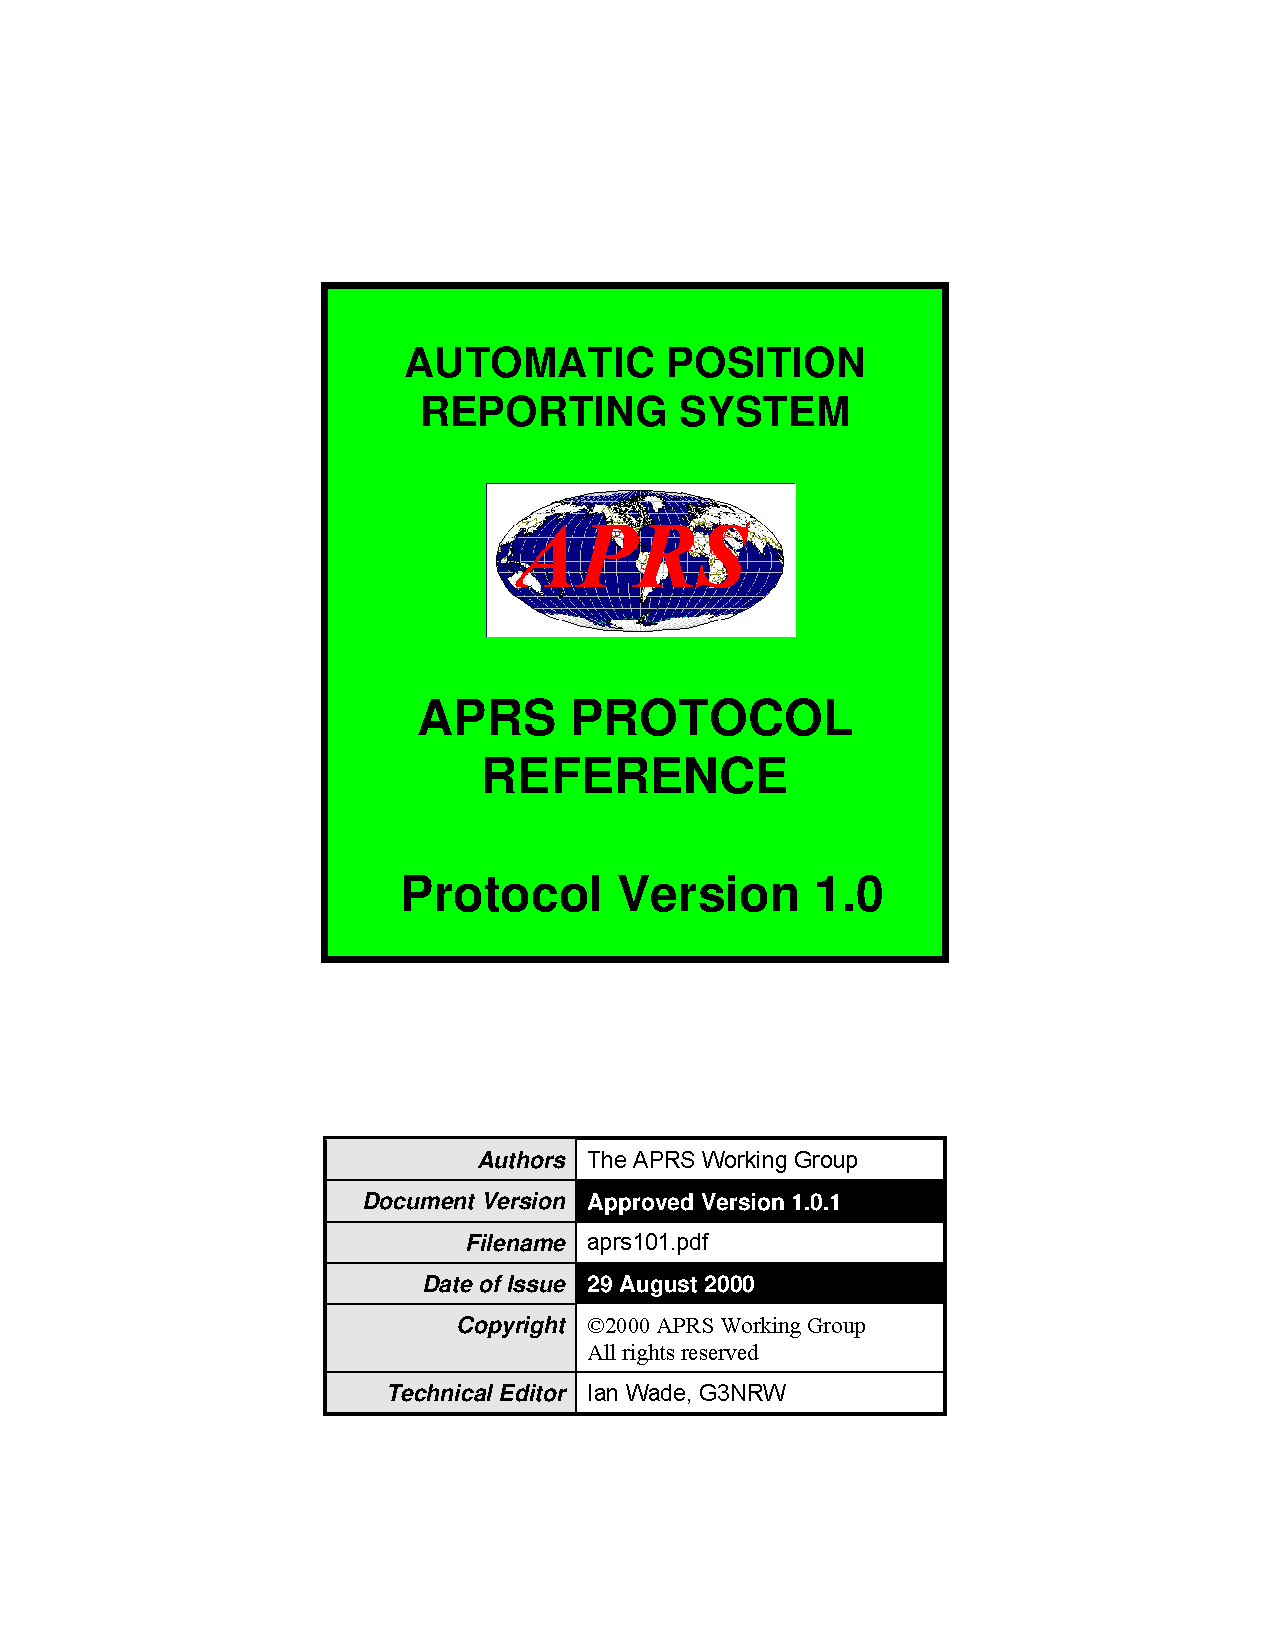
\includepdf[pages=1] {APRS101-original.pdf}

\section*{Cover Two}

\begin{verbatim}
AUTOMATIC POSITION REPORTING SYSTEM

APRS PROTOCOL REFERENCE
Protocol Version 1.0

Authors The APRS Working Group
Document Version Approved Version 1.0.1
Filename aprs101.pdf
Date of Issue 29 August 2000
Copyright ©2000 APRS Working Group
All rights reserved
Technical Editor Ian Wade, G3NRW
\end{verbatim}

\newpage

\section*{Cover Three}

\begin{verbatim}
APRS Protocol Reference
Protocol Version 1.0
by the APRS Working Group
Edited by Ian Wade

Published by
Tucson Amateur Packet Radio Corp
8987–309 East Tanque Verde Road, #337
Tucson, AZ 85749-9399
United States of America
http://www.tapr.org
ISBN 0-9644707-6-4
TAPR Publication Number: 99-4

Copyright ©2000 APRS Working Group
All rights reserved

APRS® is a registered trademark of Bob Bruninga.
WinAPRS™, MacAPRS™, X-APRS™, PalmAPRS™ and APRS/CE™
are trademarks using the APRS® name, licensed from Bob Bruninga.
This document may be copied for non-commercial purposes only, and must
include the above copyright statement and trademark statements in full.
\end{verbatim}

\newpage
\section*{Cover Four: Note on Reformatted Version}
To be added





% Part 0 Chunk 1

 % Prelude Part One

\part*{Prelude}

\section*{FOREWORD}

This APRS Protocol Reference document represents the coming-of-age of WB4APR’s baby.
Starting with a simple concept — a way to track the location of moving objects via packet radio
— programs using the APRS protocol have grown into perhaps the most popular packet radio
application in use today. It’s also become one of the most complex; from the simple idea grew,
and still grows, a tactical communications system of tremendous capability. Like many ham
projects, the APRS protocol was designed as it was being implemented, and many of its
intricacies have never been documented.

Until now. This specification defines the APRS on-air protocol with a precision and clarity that
make it a model for future efforts. The work done by members of the APRS Working Group, as
well as Technical Editor Ian Wade, G3NRW, should be recognized as a tremendous contribution
to the packet radio art. With this document available, there is now no excuse for any developer to
improperly implement the APRS protocol.

As an APRS Working Group member whose role was mainly that of observer, I was fascinated
with the interplay among the APRS authors and the Technical Editor as the specification took
form. Putting onto paper details that previously existed only in the minds of the authors exposed
ambiguities, unconsidered consequences, and even errors in what the authors thought they knew.
The discussion that followed each draft, and the questions Ian posed as he tried to wring out the
uncertainties, gave everyone a better understanding of the protocol. I am sure that this process has
already contributed to better interoperability among existing APRS applications.
Everyone who has watched the specification develop, from the initial mention in April 1999 until
release of this Version 1.0 document in August 2000, knows that the process took much longer
than was hoped. At the same time, they saw the draft transformed from a skeleton into a hefty
book of over 110 pages. With the specification now in hand, I think we can all say the wait was
worth it. Congratulations to the APRS Working Group and, in particular, to G3NRW, for a major
contribution to the literature of packet radio.

\begin{verbatim}
John Ackermann, N8UR
TAPR Vice President and APRS Working Group Administrative Chair
August 2000
\end{verbatim}


% TOC to follow


 \tableofcontents

% Part 0 Chunk 2

 \section*{Preamble}

\subsection*{APRS Working Group}

The APRS Working Group is an unincorporated association whose members
undertake to further the use and enhance the value of the APRS protocols by
(a) publishing and maintaining a formal APRS Protocol Specification; (b)
publishing validation tests and other tools to enable compliance with the
Specification; (c) supporting an APRS Certification program; and (d) generally
working to improve the capabilities of APRS within the amateur radio
community.

Although the Working Group may receive support from TAPR and other
organizations, it is an independent body and is not affiliated with any
organization. The Group has no budget, collects no dues, and owns no assets.
The current members of the APRS Working Group are:

\begin{itemize}
\item John Ackermann, N8UR Administrative Chair \& TAPR Representative
\item Bob Bruninga, WB4APR Technical Chair, founder of APRS
\item Brent Hildebrand, KH2Z Author of APRS+SA
\item Stan Horzepa, WA1LOU Secretary
\item Mike Musick, N0QBF Author of pocketAPRS
\item Keith Sproul, WU2Z Co-Author of WinAPRS/MacAPRS/X-APRS
\item Mark Sproul, KB2ICI Co-Author of WinAPRS/MacAPRS/X-APRS
\end{itemize}

\section*{Acknowledgements}
This document is the result of contributions from many people. It includes
much of the material produced by individual members of the Working
Group.

In addition, the paper on the Mic-E data format by Alan Crosswell, N2YGK,
and Ron Parsons, W5RKN was a useful starting point for explaining the
complications of this format.

\section*{Document Version Number}

Except for the very first public draft release of the APRS Protocol
Reference, the document version number is a 3-part number “P.p.D” (for
an approved document release) or a 4-part number “P.p.Dd” (for a draft
release):


% Figure/Table  Here


Thus, for example:

\begin{itemize}

\item Document version number “1.2.3” refers to document release 3 covering
APRS Protocol Version 1.2.

\item Document version number “1.2.3c” is draft “c” of that document.

\end{itemize}


\section*{Release History}

The release history for this document is listed in Appendix 7.

\section*{Document Conventions}

This document uses the following conventions:
\begin{itemize}

\item \texttt {Courier font} ASCII characters in APRS data.

\item \textvisiblespace  ASCII space character.

\item … (ellipsis) zero or more characters.

\item /\$ Symbol from Primary Symbol Table.

\item \textbackslash\$ Symbol from Alternate Symbol Table.

\item 0x hexadecimal (e.g. 0x1d).

\item All callsigns are assumed to have SSID –0 unless otherwise specified.

\item \hl{Yellow marker} (appears as light gray background in hard copy).
Marks text of interest — especially useful for highlighting single
literal ASCII characters (e.g. ") where they appear in APRS data.

\item Shaded areas in packet format diagrams are optional fields.

\end{itemize}

\section*{Feedback}

Please address your feedback or other comments regarding this document to
the TAPR aprsspec mail list.

To join the list, start at http://www.tapr.org and then follow the path Special
Interest Groups $\Rightarrow$ APRS Specification $\Rightarrow$ Join APRS Spec Discussion List.


\section*{Authors’ Foreword}

This reference document describes what is known as APRS Protocol
Version 1.0, and is essentially a description of how APRS operates
today.  It is intended primarily for the programmer who wishes to
develop APRS compliant applications, but will also be of interest to
the ordinary user who wants to know more about what goes on “under the
hood”.  It is not intended, however, to be a dry-as-dust, pedantic,
RFC-style programming specification, to be read and understood only by
the Mr Spocks of this world. We have included many items of general
information which, although strictly not part of the formal protocol
description, provide a useful background on how APRS is actually used
on the air, and how it is implemented in APRS software. We hope this
will put APRS into perspective, will make the document more readable,
and will not offend the purists too much.

It is important to realize how APRS originated, and to understand the
design philosophy behind it. In particular, we feel strongly that APRS
is, and should remain, a light-weight tactical system — almost anyone
should be able to use it in temporary situations (such as emergencies
or mobile work or weather watching) with the minimum of training and
equipment.

This document is the result of inputs from many people, and collated
and massaged by the APRS Working Group. Our sincere thanks go to
everyone who has contributed in putting it together and getting it
onto the street. If you discover any errors or omissions or misleading
statements, please let us know — the best way to do this is via the
TAPR aprsspec mailing list at www.tapr.org.

Finally, users throughout the world are continually coming up with new
ideas and suggestions for extending and improving APRS. We welcome
them.  Again, the best way to discuss these is via the aprsspec list.

--The APRS Working Group, August 2000


\section*{Disclaimer}

Like any navigation system, APRS is not infallible. No one should rely
blindly on APRS for navigation, or in life-and-death situations. Similarly,
this specification is not infallible.

The members of the APRS Working Group have done their best to define the
APRS protocol, but this protocol description may contain errors, or there
may be omissions. It is very likely that not all APRS implementations will
fully or correctly implement this specification, either today or in the future.


We urge anyone using or writing a program that implements this
specification to exercise caution and good judgement. The APRS Working
Group and the specification’s Editor disclaim all liability for injury to
persons or property that may result from the use of this specification or
software implementing it.



% Part 1 Chapter 0

 \part{The Structure of this Specification}

This specification describes the overall requirements for developing software
that complies with APRS Protocol Version 1.0. The information flow starts
with the standard AX.25 UI-frame, and progresses downwards into more and
more detail as the use of each field in the frame is explored.
A key feature of the specification is the inclusion of dozens of detailed
examples of typical APRS packets and related math computations.
Here is an outline of the chapters:

% reduce baseline skip for this section

\paragraph{Introduction to APRS --}A brief background to APRS and a summary of its
main features.

\paragraph{The APRS Design Philosophy --}The fundamentals of APRS, highlighting
its use as a real-time tactical communications tool, the timing of
APRS transmissions and the use of generic digipeating.

\paragraph{APRS and AX.25 --}A brief refresher on the structure of the AX.25
UI-frame, with particular reference to the special ways in which APRS uses
the Destination and Source Address fields and the Information field.

\paragraph{APRS Data in the AX.25 Destination and Source Address Fields --}
Details of generic APRS callsigns and callsigns that specify display symbols
and APRS software version numbers. Also a summary of how Mic-E
encoded data is stored in the Destination Address field, and how the Source
Address SSID can specify a display icon.

\paragraph{APRS Data in the AX.25 Information Field --}Details of the principal
constituents of APRS data that are stored in the Information field. Contains
the APRS Data Type Identifiers table, and a summary of all the different
types of data that the Information field can hold.

\paragraph{Time and Position Formats --}Information on formats for timestamps,
latitude, longitude, position ambiguity, Maidenhead locators, NMEA data
and altitude.

\paragraph{APRS Data Extensions --}Details of optional data extensions for station
course/speed, wind speed/direction, power/height/gain, pre-calculated radio
range, DF signal strength and Area Object descriptor.

\paragraph{Position and DF Report Data Formats --}Full details of these report
formats.

\paragraph{Compressed Position Report Data Formats --}Full details of how station
position and APRS data extensions are compressed into very short packets.

\paragraph{Mic-E Data Format --}Mic-E encoding of station lat/long position, altitude,
course, speed, Mic-E message code, telemetry data and APRS digipeater
path into the AX.25 Destination Address and Information fields.

\paragraph{Object and Item Reports --}Full information on how to set up APRS
Objects and Items, and details of the encoding of Area Objects (circles, lines,
ellipses etc).

\paragraph{Weather Reports --}Full format details for weather reports from
standalone (positionless) weather stations and for reports containing
position information. Also details of storm data format.

\paragraph{Telemetry Data --}A description of the MIM/KPC-3+ telemetry data
format, with supporting information on how to tailor the interpretation of the
raw data to individual circumstances.

\paragraph{Messages, Bulletins and Announcements --}Full format information.

\paragraph{Station Capabilities, Queries and Responses --}Details of the ten different
types of query and expected responses.

\paragraph{Status Reports --}The format of general status messages, plus the special
cases of using a status report to contain meteor scatter beam heading/power
and Maidenhead locator.

\paragraph{Network Tunneling --}The use of the Source Path Header to allow
tunneling of APRS packets through third-party networks that do not
understand AX.25 addresses, and the use of the third-party Data Type
Identifier.

\paragraph{User-Defined Data Format --}APRS allows users to define their own data
formats for special purposes. This chapter describes how to do this.

\paragraph{Other Packets --} A general statement on how APRS is to handle any other
packet types that are not covered by this specification.

\paragraph{APRS Symbols --}How to specify APRS symbols and symbol overlays, in
position reports and in generic GPS destination callsigns.

\paragraph{APRS Data Formats --}An appendix containing all the APRS data formats
collected together for easy reference.

\paragraph{The APRS Symbol Tables --}A complete listing of all the symbols in the
Primary and Alternate Symbol Tables.

\paragraph{ASCII Code Table --}The full ASCII code, including decimal and hex
codes for each character (the decimal code is needed for compressed lat/long
and altitude computations), together with the hex codes for bit-shifted ASCII
characters in AX.25 addresses (useful for Mic-E decoding and general on-air
packet monitoring).

% Note: Add Unicode Here?

\paragraph{Glossary --}A handy one-stop reference for the many APRS-specific terms
used in this specification.

\paragraph{References --}Pointers to other documents that are relevant to this
specification.

% unchange baseline skip here


% Part 1 Chapter 1

 \chapter {Chapter 1: Introduction to APRS}


\section{What is APRS?}

APRS is short for Automatic Position Reporting System, which was designed
by Bob Bruninga, WB4APR, and introduced by him at the 1992 TAPR/
ARRL Digital Communications Conference.

Fundamentally, APRS is a packet communications protocol for
disseminating live data to everyone on a network in real time. Its most visual
feature is the combination of packet radio with the Global Positioning
System (GPS) satellite network, enabling radio amateurs to automatically
display the positions of radio stations and other objects on maps on a PC.
Other features not directly related to position reporting are supported, such as
weather station reporting, direction finding and messaging.

APRS is different from regular packet in several ways:

\begin{itemize}

\item It provides maps and other data displays, for vehicle/personnel location
and weather reporting in real time.

\item It performs all communications using a one-to-many protocol, so that
everyone is updated immediately.

\item It uses generic digipeating, with well-known callsign aliases, so that prior
knowledge of network topology is not required.

\item It supports intelligent digipeating, with callsign substitution to reduce
network flooding.

\item Using AX.25 UI-frames, it supports two-way messaging and distribution
of bulletins and announcements, leading to fast dissemination of text
information.

\item It supports communications with the Kenwood TH-D7 and TM-D700
radios, which have built-in TNC and APRS firmware.

\end{itemize}

Conventional packet radio is really only useful for passing bulk message
traffic from point to point, and has traditionally been difficult to apply to
real-time events where information has a very short lifetime. APRS turns
packet radio into a real-time tactical communications and display system for
emergencies and public service applications.

APRS provides universal connectivity to all stations, but avoids the
complexity, time delays and limitations of a connected network. It permits
any number of stations to exchange data just like voice users would on a
voice net. Any station that has information to contribute simply sends it, and
all stations receive it and log it.

APRS recognizes that one of the greatest real-time needs at any special event
or emergency is the tracking of key assets. Where is the marathon leader?
Where are the emergency vehicles? What’s the weather at various points in
the county? Where are the power lines down? Where is the head of the
parade? Where is the mobile ATV camera? Where is the storm?
To address these questions, APRS provides a fully featured automatic
vehicle location and status reporting system. It can be used over any two-way
radio system including amateur radio, marine band, and cellular phone. There
is even an international live APRS tracking network on the Internet.


\section{APRS Features}

APRS runs on most platforms, including DOS, Windows 3.x, Windows
95/98, MacOS, Linux and Palm. Most implementations on these platforms
support the main features of APRS:

\begin{itemize}

\item \textbf{Maps --}APRS station positions can be plotted in real-time on maps,
with coverage from a few hundred yards to worldwide. Stations reporting
a course and speed are dead-reckoned to their present position. Overlay
databases of the locations of APRS digipeaters, US National Weather
Service sites and even amateur radio stores are available. It is possible to
zoom in to any point on the globe.


\item \textbf{Weather Station Reporting --} APRS supports the automatic display of
remote weather station information on the screen.

\item \textbf{DX Cluster Reporting --} APRS an ideal tool for the DX cluster user.
Small numbers of APRS stations connected to DX clusters can relay DX
station information to many other stations in the local area, reducing
overall packet load on the clusters.

\item \textbf{Internet Access --} The Internet can be used transparently to cross-link
local radio nets anywhere on the globe. It is possible to telnet into
Internet APRS servers and see hundreds of stations from all over the
world live. Everyone connected can feed their locally heard packets into
the APRS server system and everyone everywhere can see them.

\item \textbf{Messages --} Messages are two-way messages with acknowledgement.
All incoming messages alert the user on arrival and are held on the
message screen until killed.


\item \textbf{Bulletins and Announcements --} Bulletins and announcements are
addressed to everyone. Bulletins are sent a few times an hour for a few
hours, and announcements less frequently but possibly over a few days.

\item \textbf{Fixed Station Tracking --} In addition to automatically tracking mobile
GPS/LORAN-equipped stations, APRS also tracks from manual reports
or grid squares.

\item \textbf{Objects --} Any user can place an APRS Object on his own map, and
within seconds that object appears on all other station displays. This is
particularly useful for tracking assets or people that are not equipped
with trackers. Only one packet operator needs to know where things are
(e.g. by monitoring voice traffic), and as he maintains the positions and
movements of assets on his screen, all other stations running APRS will
display the same information.


\end{itemize}


% Part 1 Chapter 2

 \chapter{Chapter 2: APRS Design Philosophy}


\section{Net Cycle Time}

It is important to note that APRS is primarily a real-time, tactical
communications tool, to help the flow of information for things like special
events, emergencies, Skywarn, the Emergency Operations Center and just
plain in-the-field use under stress. But like the real world, for 99\% of the
time it is operating routinely, waiting for the unlikely serious event to
happen.

Anything which is done to enhance APRS must not undermine its ability to
operate in local areas under stress. Here are the details of that philosophy:

\begin {enumerate}

\item APRS uses the concept of a “net cycle time”. This is the time within
which a user should be able to hear (at least once) all APRS stations
within range, to obtain a more or less complete picture of APRS activity.
The net cycle time will vary according to local conditions and with the
number of digipeaters through which APRS data travels.

\item The objective is to have a net cycle time of 10 minutes for local use. This
means that within 10 minutes of arrival on the scene, it is possible to
captured the entire tactical picture.

\item  All stations, even fixed stations, should beacon their position at the net
cycle time rate. In a stress situation, stations are coming and going all the
time. The position reports show not only where stations are without
asking, but also that they are still active.

\item It is not reasonable to assume that all APRS users responding to a stress
event understand the ramifications of APRS and the statistics of the
channel — user settings cannot be relied on to avoid killing a stressed
net. Thus, to try to anticipate when the channel is under stress, APRS
automatically adjusts its net cycle time according to the number of
digipeaters in the UNPROTO path:

\begin{itemize}

\item Direct operation (no digipeaters): 10 minutes (probably an
event).

\item Via one digipeater hop: 10 minutes (probably an event).

\item Via two digipeater hops: 20 minutes.

\item Via three or more digipeater hops: 30 minutes.

\end{itemize}

\item Since almost all home stations set their paths to three or more
digipeaters, the default net cycle time for routine daily operation is
30 minutes. This should be a universal standard that everyone can bank
on -- if you routinely turn on your radio and APRS and do nothing
else, then in 30 minutes you should have virtually the total picture
of all APRS stations within range.

\item Since knowing where the digipeaters are located is fundamental to APRS
connectivity, digipeaters should use multiple beacon commands to
transmit position reports at different rates over different paths; i.e. every
10 minutes for sending position reports locally, and every 30 minutes for
sending them via three digipeaters (plus others rates and distances as
needed).

\item If the net cycle time is too long, users will be tempted to send queries for
APRS stations. This will increase the traffic on the channel
unnecessarily. Thus the recommended extremes for net cycle time are 10
and 30 minutes — this gives network designers the fundamental
assumptions for channel loading necessary for good engineering design.

\end{enumerate}

\section {Packet Timing}

Since APRS packets are error-free, but are not guaranteed delivery, APRS
transmits information redundantly. To assure rapid delivery of new or
changing data, and to preserve channel capacity by reducing interference
from old data, APRS should transmit new information more frequently than
old information.

There are several algorithms in use to achieve this:

\begin{itemize}


\item \textbf{Decay Algorithm --} Transmit a new packet once and n seconds later.
Double the value of n for each new transmission. When n reaches the
net cycle time, continue at that rate. Other factors besides
“doubling” may be appropriate, such as for new message lines.

\item \textbf{Fixed Rate --} Transmit a new packet once and n seconds later. Transmit
it x times and stop.

\item \textbf{Message-on-Heard --} Transmit a new packet according to either
algorithm above. If the packet is still valid, and has not been
acknowledged, and the net cycle time has been reached, then the
recipient is probably not available. However, if a packet is then
subsequently heard from the recipient, try once again to transmit the
packet.

\item \textbf{Time-Out --} This term is used to describe a time period beyond which it
is reasonable to assume that a station no longer exists or is off the air if
no packets have been heard from it. A period of 2 hours is suggested as
the nominal default timeout. This time-out is not used in any transmitting
algorithms, but is useful in some programs to decide when to cease
displaying stations as “active”. Note that on HF, signals come and go, so
decisions about activity may need to be more flexible.


\end{itemize}

\section{Generic Digipeating}


The power of APRS in the field derives from the use of generic digipeating,
in that packets are propagated without a priori knowledge of the network.
There are six powerful techniques which have evolved since APRS was
introduced in 1992:

\begin{enumerate}

\item \textbf{RELAY --} Every VHF APRS TNC is assumed to have an alias of
RELAY, so that anyone can use it as a digipeater at any time.

\item \textbf{ECHO --} HF stations use the alias of ECHO as an alternative to
RELAY. (However, bearing in mind the nature of HF propagation, this
has the potential of causing interference over a wide area, and should
only be used sparingly by mobile stations).

\item \textbf{WIDE --} Every high-site digipeater is assumed to have an alias of WIDE
for longer distance communications.

\item \textbf{TRACE --} Every high-site digipeater that is using callsign substitution
is assumed to have the alias of TRACE. These digipeaters self-identify
packets they digipeat by inserting their own call in place of RELAY,
WIDE or TRACE.

\item \textbf{WIDEn-N --} A digipeater that supports WIDEn-N digipeating will
digipeat any WIDEn-N packet that is “new” and will subtract 1 from the
SSID until the SSID reaches –0. The digipeater keeps a copy or a
checksum of the packet and will not digipeat that packet again within
(typically) 28 seconds. This considerably reduces the number of
superfluous digipeats in areas with many digipeaters in radio range of
each other.

\item \textbf{GATE --} This generic callsign is used by HF-to-VHF Gateway
digipeaters. Any packet heard on HF via GATE will be digipeated locally
on VHF. This permits local networks to keep an eye on the national and
international picture.

\end{enumerate}

\section{Communicating Map Views Unambiguously}

APRS is a tactical geographical system. To maximize its operational
effectiveness and minimize confusion between operators of different
systems, users need to have an unambiguous way to communicate to others
the “location” and “size” (or area of coverage) of any map view.
The APRS convention is by reference to a center and range which specify
the geographical center and approximate radius of a circle that will fit in the
map view independent of aspect ratio. The radius of the circle (in nautical
miles, statute miles or km) is known as the “range scale”. This convention
gives all users a simple common basis for describing any specific map view
to others over any communications medium or program.


% Part 1 Chapter 3

\chapter{Chapter 3: APRS and AX.25}


\section{Protocols}

At the link level, APRS uses the AX.25 protocol, as defined in Amateur
Packet-Radio Link-Layer Protocol (see Appendix 6 for details), utilizing
Unnumbered Information (UI) frames exclusively. This means that APRS
runs in connectionless mode, whereby AX.25 frames are transmitted without
expecting any response, and reception at the other end is not guaranteed.
At a higher level, APRS supports a messaging protocol that allows users to
send short messages (one line of text) to nominated stations, and expects to
receive acknowledgements from those stations.

\subsection{The AX.25 Frame}

\begin{center}
All APRS transmissions use AX.25 UI-frames, with 9 fields of data:
\end{center}

\begin{tabular}{|l|c|c|c|c|c|c|c|c|c|}
  \hline
  \multicolumn{10}{|c|}{AX.25 UI-FRAME FORMAT} \\
  \hline
  \hline 
  FIELD & Flag & Destination & Source & Digipeater  & Control & Protocol  & Information  & FCS & Flag \\
  NAME & & Address & Address & Addresses & Field  & ID & Field &  &    \\
  &         &         &    & (0--8)     & (UI)   &       &  &  &  \\
  \hline
  BYTES & 1  & 7  & 7  & 0--56 & 1  & 1  & 1--256  & 2  & 1 \\
  \hline
  
  FIELD & One & Two & Three & Four & Five & Six & Seven & Eight & Nine \\
  NUMBER  &     &     &       &      &      &     &       &       &      \\
  
  \hline
\end{tabular}

\begin{itemize}


\item \textbf{Flag--} The flag field at each end of the frame is the bit sequence 0x7e
that separates each frame.

\item \textbf{Destination Address--} This field can contain an APRS destination
callsign or APRS data. APRS data is encoded to ensure that the field
conforms to the standard AX.25 callsign format (i.e. 6 alphanumeric
characters plus SSID). If the SSID is non-zero, it specifies a generic
APRS digipeater path.

\item \textbf{Source Address--} This field contains the callsign and SSID of the
transmitting station. In some cases, if the SSID is non-zero, the SSID
may specify an APRS display Symbol Code.

\item \textbf{Digipeater Addresses--} From zero to 8 digipeater callsigns may be
included in this field. Note: These digipeater addresses may be
overridden by a generic APRS digipeater path (specified in the
Destination Address SSID).

\item \textbf{Control Field--} This field is set to 0x03 (UI-frame).

\item \textbf{Protocol ID--} This field is set to 0xf0 (no layer 3 protocol).

\item \textbf{Information Field--} This field contains more APRS data. The first
character of this field is the APRS Data Type Identifier that specifies the
nature of the data that follows.

\item \textbf{Frame Check Sequence--} The FCS is a sequence of 16 bits used for
  checking the integrity of a received frame.

\item \textbf{Flag--} The flag field at each end of the frame is the
  bit sequence 0x7e that separates each frame.
    

\end{itemize}


% Part 1 Chapter 4

\chapter{Chapter 4: APRS Data in the AX.25 Destination and Source Address Fields}


\section{The AX.25 Destination Address Field}

The AX.25 Destination Address field can contain 6 different types of APRS
information:

\begin{itemize}

\item A generic APRS address.

\item A generic APRS address with a symbol.

\item An APRS software version number.

\item Mic-E encoded data.

\item A Maidenhead Grid Locator (obsolete).

\item An Alternate Net (ALTNET) address.

\end{itemize}

In all of these cases, the Destination Address SSID may specify a generic
APRS digipeater path.

\section {Generic APRS Destination Addresses}

APRS uses the following generic beacon-style destination addresses:

% Start Chart

AIR* †
DGPS*
QST*
TEL*

ALL*
DRILL*
QTH*
TEST*

AP*
DX*
RTCM*
TLM*

BEACON
ID*
SKY*
WX*

CQ*
GPS*
JAVA* MAIL*
SPACE* SPC*
ZIP* †

DF*
MICE*
SYM*

% End chart

The asterisk is a wildcard, allowing the address to be extended (up to a total
of 6 alphanumeric characters). Thus, for example, WX1, WX12 and WX12CD
are all valid APRS destination addresses.
† The AIR* and ZIP* addresses are being phased out, but are needed at
present for backward compatibility.

All of these addresses have an SSID of –0. Non-zero SSIDs are reserved for
generic APRS digipeating.

These addresses are copied by everyone. All APRS software must accept
packets with these destination addresses.

The address GPS (i.e. the 3-letter address GPS, not GPS*) is specifically
intended for use by trackers sending lat/long positions via digipeaters which
have the capability of converting positions to compressed data format.

The addresses DGPS and RTCM are used by differential GPS correction
stations. Most software will not make use of packets using this address, other
than to pass them on to an attached GPS unit.

The address SKY is used for Skywarn stations.

Packets addressed to SPCL are intended for special events. APRS software
can display such packets to the exclusion of all others, to minimize clutter on
the screen from other stations not involved in the special event.

The addresses TEL and TLM is used for telemetry stations.

\section{Generic APRS Address with Symbol}

APRS uses several of the above-listed generic addresses in a special way, to
specify not only an address but also a display symbol. These special
addresses are GPSxyz, GPSCnn, GPSEnn, SPCxyz and SYMxyz, and are
intended for use where it is not possible to include the symbol in the AX.25
Information field.

The GPS addresses above are for general use.
The SPC addresses are intended for special events.
The SYM addresses are reserved for future use.
The characters xy and nn refer to entries in the APRS Symbol Tables. The
character z specifies a symbol overlay. See Chapter 20: APRS Symbols and
Appendix 2 for more information.

\section{APRS Software Version Number}

The AX.25 Destination Address field can contain the version number of the
APRS software that is running at the station. Knowledge of the version
number can be useful when debugging.
The following software version types are reserved (xx and xxx indicate a
version number):

\begin{itemize}

\item APCxxx APRS/CE, Windows CE
\item APDxxx Linux aprsd server
\item APExxx PIC-Encoder
\item APIxxx Icom radios (future)
\item APICxx ICQ messaging
\item APKxxx Kenwood radios
\item APMxxx MacAPRS
\item APPxxx pocketAPRS
\item APRxxx APRSdos
\item APRS older versions of APRSdos
\item APRSM older versions of MacAPRS
\item APRSW older versions of WinAPRS
\item APSxxx APRS+SA
\item APWxxx WinAPRS
\item APXxxx X-APRS
\item APYxxx Yaesu radios (future)
\item APZxxx Experimental

\end{itemize}

This table will be added to by the APRS Working Group.
For example, a station using version 3.2.6 of MacAPRS could use the
destination callsign \texttt{APM326}.

The Experimental destination is designated for temporary use only while a
product is being developed, before a special APRS Software Version address
is assigned to it.


\section {Mic-E Encoded Data}

Another alternative use of the AX.25 Destination Address field is to contain
Mic-E encoded data. This data includes:

\begin{itemize}

\item The latitude of the station.

\item A West/East Indicator and a Longitude Offset Indicator (used in
longitude computations).

\item A Message Code.

\item The APRS digipeater path.

\end{itemize}
This data is used with associated data in the AX.25 Information field to
provide a complete Position Report and other information about the station
(see Chapter 10: Mic-E Data Format).

\section {Maidenhead Grid Locator in Destination Address}

The AX.25 Destination Address field may contain a 6-character Maidenhead
Grid Locator. For example: IO91SX. This format is typically used by meteor
scatter and satellite operators who need to keep packets as short as possible.

This format is now obsolete.

\section{Alternate Nets}

Any other destination address not included in the specific generic list or the
other categories mentioned above may be used in Alternate Nets (ALTNETs)
by groups of individuals for special purposes. Thus they can use the APRS
infrastructure for a variety of experiments without cluttering up the maps and
lists of other APRS stations. Only stations using the same ALTNET address
should see their data.

\section{Generic APRS Digipeater Path}


The SSID in the Destination Address field of all packets is coded to specify
the APRS digipeater path.

If the Destination Address SSID is –0, the packet follows the standard AX.25
digipeater (“VIA”) path contained in the Digipeater Addresses field of the
AX.25 frame.

If the Destination Address SSID is non-zero, the packet follows one of 15
generic APRS digipeater paths.


The SSID field in the Destination Address (i.e. in the 7th address byte) is
encoded as follows:

% Chart start

APRS Digipeater Paths in Destination Address SSID
SSID

The AX.25 Source
Address SSID to
specify Symbols

Path

-0

Use VIA path

-1
-2

SSID

Path

-8

North path

WIDE1-1

-9

South path

WIDE2-2

-10

East path

-3

WIDE3-3

-11

West path

-4

WIDE4-4

-12

North path + WIDE

-5

WIDE5-5

-13

South path + WIDE

-6

WIDE6-6

-14

East path + WIDE

-7

WIDE7-7

-15

West path + WIDE

% end chart

\section{The AX.25 Source Address SSID to specify Symbols}

The AX.25 Source Address field contains the callsign and SSID of the
originating station. If the SSID is –0, APRS does not treat it in any special
way.

If, however, the Source Address SSID is non-zero, APRS interprets it as a
display icon. This is intended for use only with stand-alone trackers where
there is no other method of specifying a display symbol or a destination
address (e.g. MIM trackers or NMEA trackers).

For more information, see Chapter 20: APRS Symbols.


% Part 1 Chapter 5

\chapter {Chapter 5: APRS Data in the AX.25 Information Field}

\section {Generic Data Format}

In general, the AX.25 Information field can contain some or all of the
following information:
\begin{itemize}
\item  APRS Data Type Identifier
\item  APRS Data
\item  APRS Data Extension
\item  Comment
\end{itemize}

% begin chart

\begin{tabular}{|l|c|c|c|c|}
  \hline
  \hline
  \multicolumn{5}{|l|}{Generic APRS Information Field} \\
  \hline
  & Data Type ID & APRS Data & APRS Data Extension & Comment \\
  \hline 
  Bytes: & 1            & n         & 7                   & n \\
  \hline
\end{tabular}


% end chart

\section{APRS Data Type Identifier}

Every APRS packet contains an APRS Data Type Identifier (DTI). This
determines the format of the remainder of the data in the Information field, as
follows:

% begin chart

\begin{verbatim}
APRS Data Type Identifiers
Ident

Data Type

Ident

Data Type

0x1c

Current Mic-E Data (Rev 0 beta)

<

Station Capabilities

0x1d

Old Mic-E Data (Rev 0 beta)

=

Position without timestamp (with APRS
messaging)

!

Position without timestamp (no APRS
messaging), or Ultimeter 2000 WX Station

>

Status

"

[Unused]

?

Query

#

Peet Bros U-II Weather Station

@

Position with timestamp (with APRS messaging)

$

Raw GPS data or Ultimeter 2000

%

Agrelo DFJr / MicroFinder

&

[Reserved — Map Feature]

'

Old Mic-E Data (but Current data for TM-D700)

[

Maidenhead grid locator beacon (obsolete)

(

[Unused]

\

[Unused]

)

Item

]

[Unused]

*

Peet Bros U-II Weather Station

^

[Unused]

+

[Reserved — Shelter data with time]

_

Weather Report (without position)

,

Invalid data or test data

‘

-

[Unused]

.

[Reserved — Space weather]

{

User-Defined APRS packet format

/

Position with timestamp (no APRS messaging)

|

[Do not use — TNC stream switch character]

[Do not use]

}

Third-party traffic

:

Message

~

[Do not use — TNC stream switch character]

;

Object

0–9

A–S
T
U–Z

a–z



[Do not use]
Telemetry data
[Do not use]

Current Mic-E Data (not used in TM-D700)
[Do not use]

\end{verbatim}

% end chart




\textbf{Note:} There is one exception to the requirement for the Data Type Identifier
to be the first character in the Information field — this is the Position without
Timestamp (indicated by the ! DTI). The ! character may occur anywhere
up to and including the 40th character position in the Information field. This
variability is required to support X1J TNC digipeaters which have a string of
unmodifiable text at the beginning of the field.

% footnote that this exception was later removed in spec version 1.1 (check)

\textbf{Note:} The Kenwood TM-D700 radio uses the ' DTI for current Mic-E data.
The radio does not use the ‘ DTI.

\section{APRS Data and Data Extension}



There are 10 main types of APRS Data:

\begin {itemize}

\item Position
\item Direction Finding
\item Objects and Items
\item Weather
\item Telemetry
\item Messages, Bulletins and Announcements
\item Queries
\item Responses
\item Status
\item Other

\end{itemize}

Some of this data may also have an APRS Data Extension that provides
additional information.

The APRS Data and optional Data Extension follow the Data Type Identifier.
The table on the next page shows a complete list of all the different possible
types of APRS Data and APRS Data Extension.



Possible APRS Data

Possible APRS Data Extension

Time (DHM or HMS)
Lat/long coordinates
Compressed lat/long/course/speed/radio range/altitude
Symbol Table ID and Symbol Code
Mic-E longitude, speed and course, telemetry or status
Raw GPS NMEA sentence
Raw weather station data

Course and Speed
Power, Effective Antenna Height/Gain/Directivity
Pre-Calculated Radio Range
Omni DF Signal Strength
Storm Data (in Comment field)

Time (DHM or HMS)
Lat/long coordinates
Compressed lat/long/course/speed/radio range/altitude
Symbol Table ID and Symbol Code

Course and Speed
Power, Effective Antenna Height/Gain/Directivity
Pre-Calculated Radio Range
Omni DF Signal Strength
Bearing and Number/Range/Quality
(in Comment field)

Objects and
Items

Object name
Item name
Time (DHM or HMS)
Lat/long coordinates
Compressed lat/long/course/speed/radio range/altitude
Symbol Table ID and Symbol Code
Raw weather station data

Course and Speed
Power, Effective Antenna Height/Gain/Directivity
Pre-Calculated Radio Range
Omni DF Signal Strength
Area Object
Storm Data (in Comment field)
Wind Direction and Speed
Storm Data (in Comment field)

Weather

Time (MDHM)
Lat/long coordinates
Compressed lat/long/course/speed/radio range/altitude
Symbol Table ID and Symbol Code
Raw weather station data

Position

Direction Finding

Telemetry
Messages,
Bulletins and
Announcements

Queries

Responses

Status

Other

Telemetry (non Mic-E)
Addressee
Message Text
Message Identifier
Message Acknowledgement
Bulletin ID, Announcement ID
Group Bulletin ID
Query Type
Query Target Footprint
Addressee (Directed Query)
Position
Object/Item
Weather
Status
Message
Digipeater Trace
Stations Heard
Heard Statistics
Station Capabilities

Course and Speed
Power, Effective Antenna Height/Gain/Directivity
Pre-Calculated Radio Range
Omni DF Signal Strength
Area Object
Wind Direction and Speed

Time (DHM zulu)
Status text
Meteor Scatter Beam Heading/Power
Maidenhead Locator (Grid Square)
Altitude (Mic-E)
E-mail message
Third-Party forwarding
Invalid Data/Test Data


\section{Comment Field}

In general, any APRS packet can contain a plain text comment (such as a
beacon message) in the Information field, immediately following the APRS
Data or APRS Data Extension.

There is no separator between the APRS data and the comment unless
otherwise stated.

The comment may contain any printable ASCII characters (except | and ~,
which are reserved for TNC channel switching).

The maximum length of the comment field depends on the report — details
are included in the description of each report.

In special cases, the Comment field can also contain further APRS data:

\begin{itemize}


\item Altitude in comment text (see Chapter 6: Time and Position Formats), or
in Mic-E status text (see Chapter 10: Mic-E Data Format).

\item Maidenhead Locator (grid square), in a Mic-E status text field (see
Chapter 10: Mic-E Data Format) or in a Status Report (see Chapter 16:
Status Reports).

\item Bearing and Number/Range/Quality parameters (/BRG/NRQ), in DF
reports (see Chapter 7: APRS Data Extensions).

\item Area Object Line Widths (see Chapter 11: Object and Item Reports).

\item Signpost Objects (see Chapter 11: Object and Item Reports).

\item Weather and Storm Data (see Chapter 12: Weather Reports).

\item Beam Heading and Power, in Status Reports (see Chapter 16: Status
Reports).

\end{itemize}

\section{Base-91 Notation}

Two APRS data formats use base-91 notation: lat/long coordinates in
compressed format (see Chapter 9) and the altitude in Mic-E format (see
Chapter 10).

Base-91 data is compressed into a short string of characters. All the
characters are printable ASCII, with character codes in the range 33–124
decimal (i.e. ! through |).

To compute the base-91 ASCII character string for a given data value, the
value is divided by progressively reducing powers of 91 until the remainder
is less than 91. At each step, 33 is added to the modulus of the division
process to obtain the corresponding ASCII character code.

For example, for a data value of 12345678:
\begin{verbatim}
12345678 / 91^3 = modulus 16, remainder 288542
288542 / 91^2 = modulus 34, remainder 6988
6988 / 91^1 = modulus 76, remainder 72
\end{verbatim}

The four ASCII character codes are thus 49 (i.e. 16+33), 67 (i.e. 34+33), 109
(i.e. 76+33) and 105 (i.e. 72+33), corresponding to the ASCII string 1Cmi.

\section{APRS Data Units}

For historical reasons there is some lack of consistency between units of data
in APRS packets — some speeds are in knots, others in miles per hour; some
altitudes are in feet, others in meters, and so on. It is emphasized that this
specification describes the units of data as they are transmitted on-air. It is
the responsibility of APRS applications to convert the on-air units to more
suitable units if required.

The default GPS earth datum is World Geodetic System (WGS) 1984.





% Part 1 Chapter 6
\chapter{Chapter 6: Time and Position Formats}


\section{Time Formats}

APRS timestamps are expressed in three different ways:

\begin{itemize}
\item Day/Hours/Minutes format
\item Hours/Minutes/Seconds format
\item Month/Day/Hours/Minutes format
\end{itemize}

In all three formats, the 24-hour clock is used.

{\bf Day/Hours/Minutes} (DHM) format is a fixed 7-character field,
consisting of a 6-digit day/time group followed by a single time
indicator character (z or /). The day/time group consists of a
two-digit day-of-the-month (01–31) and a four-digit time in hours and
minutes.

Times can be expressed in {\it zulu} (UTC/GMT) or local time. For example:

\begin{verbatim}
092345z  is 2345 hours zulu time on the 9th day of the month. 
092345/  is 2345 hours local time on the 9th day of the month. 
\end{verbatim}
 
It is recommended that future APRS implementations only transmit zulu
format on the air.

Note: The time in Status Reports may only be in zulu format.

Hours/Minutes/Seconds (HMS) format is a fixed 7-character field,
consisting of a 6-digit time in hours, minutes and seconds, followed by the h
time-indicator character. For example:

234517h is 23 hours 45 minutes and 17 seconds zulu.

Note: This format may not be used in Status Reports.

Month/Day/Hours/Minutes (MDHM) format is a fixed 8-character field,
consisting of the month (01–12) and day-of-the-month (01–31), followed by
the time in hours and minutes zulu. For example:

10092345 is 23 hours 45 minutes zulu on October 9th.

This format is only used in reports from stand-alone “positionless” weather
stations (i.e. reports that do not contain station position information).

\section{Use of Timestamps}

When a station transmits a report without a timestamp, an APRS receiving
station can make an internal record of the time it was received, if required.
This record is the receiving station’s notion of the time the report was
created.

On the other hand, when a station transmits a report with a timestamp, that
timestamp represents the transmitting station’s notion of the time the report
was created.

In other words, reports sent without a timestamp can be regarded as
real-time, “current” reports (and the receiving station has to record
the time they were received), whereas reports sent with a timestamp
may or may not be realtime, and may possibly be (very) “old”.

Four APRS Data Type Identifiers specify whether or not a report
contains a timestamp, depending on whether the station has APRS
messaging capability or not:

% Chart here


No APRS
Messaging

With APRS
Messaging

(Current/real-time)

Report without timestamp

!

=

(Old/non-real-time)

Report with timestamp

/

@

Stations without APRS messaging capability are typically stand-alone
trackers or digipeaters. Stations reporting without a timestamp are generally
(but not necessarily) fixed stations.

\section{Latitude Format}

Latitude is expressed as a fixed 8-character field, in degrees and decimal
minutes (to two decimal places), followed by the letter N for north or S for
south.

Latitude degrees are in the range 00 to 90. Latitude minutes are expressed as
whole minutes and hundredths of a minute, separated by a decimal point.

For example:
4903.50N

is 49 degrees 3 minutes 30 seconds north.

In generic format examples, the latitude is shown as the 8-character string
ddmm.hhN (i.e. degrees, minutes and hundredths of a minute north).

\section{Longitude Format}

Longitude is expressed as a fixed 9-character field, in degrees and decimal
minutes (to two decimal places), followed by the letter E for east or W for
west.


Longitude degrees are in the range 000 to 180. Longitude minutes are
expressed as whole minutes and hundredths of a minute, separated by a
decimal point.

For example:

07201.75W is 72 degrees 1 minute 45 seconds west.

In generic format examples, the longitude is shown as the 9-character string
dddmm.hhW (i.e. degrees, minutes and hundredths of a minute west).

\section{Position Coordinates}

Position coordinates are a combination of latitude and longitude, separated
by a display Symbol Table Identifier, and followed by a Symbol Code. For
example:

4903.50N/07201.75W-

The / character between latitude and longitude is the Symbol Table
Identifier (in this case indicating use of the Primary Symbol Table), and the –
character at the end is the Symbol Code from that table (in this case,
indicating a “house” icon).

A description of display symbols is included in Chapter 20: APRS Symbols.
The full Symbol Table listing is in Appendix 2.

\section{Position Ambiguity}

% Need to fix the V thing here

In some instances — for example, where the exact position is not known —
the sending station may wish to reduce the number of digits of precision in
the latitude and longitude. In this case, the mm and hh digits in the latitude
may be progressively replaced by a \textvisiblespace (space) character as the amount of
imprecision increases. For example:

\begin{description}
 
\item 4903.5\textvisiblespace N represents latitude to nearest 1/10th of a minute.
\item 4903.\textvisiblespace\textvisiblespace N represents latitude to nearest minute.
\item 490\textvisiblespace.\textvisiblespace\textvisiblespace N represents latitude to nearest 10 minutes.
\item 49\textvisiblespace\textvisiblespace.\textvisiblespace\textvisiblespace N represents latitude to nearest degree.
\end{description}

The level of ambiguity specified in the latitude will automatically apply to
the longitude as well — it is not necessary to include any \textvisiblespace characters in the
longitude.

For example, the coordinates:

4903.VVN/07201.75W- represent the position to the nearest minute. That
is, the hundredths of minutes of latitude and longitude may take any
value in the range 00–99.

Thus the station may be located anywhere inside a bounding box having the
following corner coordinates:

\begin{itemize}

\item North West corner: 49 deg 3.99 mins N, 72 deg 1.99 mins W
\item North East corner: 49 deg 3.99 mins N, 72 deg 1.00 mins W
\item South East corner: 49 deg 3.00 mins N, 72 deg 1.00 mins W
\item South West corner: 49 deg 3.00 mins N, 72 deg 1.99 mins W

\end{itemize}

\section{Default Null Position}

Where a station does not have any specific position information to transmit
(for example, a Mic-E unit without a GPS receiver connected to it), the
station must transmit a default null position in the location field.

The null position corresponds to 0° 0' 0" north, 0° 0' 0" west.  The
null position should be {\it(sic)} include the \. symbol
(unknown/indeterminate position).

For example, a Position Report for a station with unknown position
will contain the coordinates:

\begin{verbatim}
…0000.00N\00000.00W.…
\end{verbatim}

\section{Maidenhead Locator (Grid Square)}

An alternative method of expressing a station’s location is to provide a
Maidenhead locator (grid square). There are four ways of doing this:

\begin{itemize}
  
\item In a Status Report — e.g. IO91SX/(/- represents the symbol for a “house”).

\item In Mic-E Status Text — e.g. IO91SX/G
(/G indicates a “grid square”).

\item In the Destination Address — e.g. IO91SX. (obsolete).

\item In AX.25 beacon text, with the [ APRS Data Type Identifier — e.g.
[IO91SX] (obsolete).

\end{itemize}

Grid squares may be in 6-character form (as above) or in the shortened
4-character form (e.g. IO91).

\section{NMEA Data}

APRS recognizes raw ASCII data strings conforming to the NMEA 0183
Version 2.0 specification, originating from navigation equipment such as
GPS and LORAN receivers. It is recommended that APRS stations interpret
at least the following NMEA Received Sentence types:

\begin{itemize}

\item GGA Global Positioning System Fix Data
\item GLL Geographic Position, Latitude/Longitude Data
\item RMC Recommended Minimum Specific GPS/Transit Data
\item VTG Velocity and Track Data
\item WPT Way Point Location
% footnote WPT as typo, as mentioned in 1.1


\end{itemize}



\section{Altitude}

Altitude may be expressed in two ways:

\begin{itemize}
\item In the comment text.
\item In Mic-E format.
\end{itemize}

\textbf{Altitude in Comment Text --} The comment may contain an altitude value,
in the form /A=aaaaaa, where aaaaaa is the altitude in feet. For example:
/A=001234. The altitude may appear anywhere in the comment.

\textbf{Altitude in Mic-E format --} The optional Mic-E status field can contain
altitude data. See Chapter 10: Mic-E Data Format.



% Part 1 Chapter 7

\chapter{Chapter 7: APRS Data Extensions}


A fixed-length 7-byte field may follow APRS position data. This field is an
APRS Data Extension. The extension may be one of the following:

\section{Course and Speed}

\begin{tabular}{p{0.25\linewidth}  p{0.6\linewidth}}

 CSE/SPD & Course and Speed (this may be followed by a further 8 bytes
 containing DF bearing and Number/Range/Quality parameters) \\
  & \\
 DIR/SPD & Wind Direction and Wind Speed \\
  & \\
 PHGphgd & Station Power and Effective Antenna Height/Gain/
Directivity \\
  & \\
 RNGrrrr & Pre-Calculated Radio Range \\
  & \\
 DFSshgd & DF Signal Strength and Effective Antenna Height/Gain \\
  & \\
 Tyy/Cxx & Area Object Descriptor \\
 & \\
 & \\
\end{tabular}


The 7-byte CSE/SPD Data Extension can be used to represent the course and
speed of a vehicle or APRS Object.
The course is expressed in degrees (001-360), clockwise from due north. The
speed is expressed in knots. A slash / character separates the two.

For example:
088/036 represents a course 88 degrees, traveling at 36 knots.

If the course and speed are unknown or not relevant, they can be set
to 000/000 or
.../... or \textvisiblespace \textvisiblespace \textvisiblespace
/\textvisiblespace \textvisiblespace \textvisiblespace .

Note: In the special case of DF reports, a course of 000 means that the DF
station is fixed. If the course is non-zero, the station is mobile.

\section {Wind Direction and Wind Speed}

The 7-byte DIR/SPD Data Extension can be used to represent the wind
direction and sustained one-minute wind speed in a Weather Report.
The wind direction is expressed in degrees (001-360), clockwise from due
north. The speed is expressed in knots. A slash / character separates the two.

For example:

220/004 represents a wind direction of 220 degrees and a speed of 4 knots.

If the wind direction and speed are unknown or not relevant, they can be set
to 000/000 or .../... or  \textvisiblespace \textvisiblespace \textvisiblespace
/\textvisiblespace \textvisiblespace \textvisiblespace .

\section{Power, Effective Antenna Height/Gain/Directivity}

The 7-byte PHGphgd Data Extension specifies the transmitter power,
effective antenna height-above-average-terrain, antenna gain and antenna
directivity. APRS uses this information to plot radio range circles around
stations.


The 7 characters of this Data Extension are encoded as follows:

\begin{tabular}{lcr}

Characters 1–3: & PHG & (fixed) \\

Character 4: & p & Power code \\

Character 5: & h & Height code \\

Character 6: & g & Antenna gain code \\

Character 7: & d & Directivity code \\

& \\
& \\
\end{tabular}



% Start Chart


The PHG codes are listed in the table below:
\begin{table}
  \caption {PHG Codes}
  \begin{tabular}{|c|c|c|c|c|c|c|c|c|c|c|c|}
    \hline      
    phgd Code: & 0 & 1 & 2 & 3 & 4 & 5 & 6 & 7 & 8 & 9 & Units \\
    \hline  
    Power & 0 & 1 & 4 & 9 & 16 & 25 & 36 & 49 & 64 & 81 & watts \\
    \hline  
    Height & 10 & 20 & 40 & 80 & 160 & 320 & 640 & 1280 & 2560 & 5120 & feet \\
    \hline  
    Gain & 0 & 1 & 2 & 3 & 4 & 5 & 6 & 7 & 8 & 9 & dB \\
    \hline  
    Directivity & omni & 45 NE & 90 E & 135 SE & 180 S & 225 SW & 270 W & 315 NW & 360 N & & deg \\
    \hline  
  \end{tabular}
\end{table}


% End Chart

The height code represents the effective height of the antenna above average
local terrain, not above ground or sea level — this is to provide a rough
indication of the antenna’s effectiveness in the local area.

The height code may in fact be any ASCII character 0–9 and above. This is
so that larger heights for balloons, aircraft or satellites may be specified.

For example:
\begin{itemize}
  
\item : is the height code for 10240 feet (approximately 1.9 miles).
\item ; is the height code for 20480 feet (approximately 3.9 miles), and so on.
\end{itemize}

The Directivity code offsets the PHG circle by one third in the indicated
direction. This means a front-to-back ratio of 2 to 1. Most often this is used
to indicate a favored direction or a null, even if an omni antenna is at the site.

An example of the PHG Data Extension:

\begin{itemize}
\item PHG5132
\end{itemize}

\begin{itemize}
% means

\item a power of 25 watts,
\item an antenna height of 20 feet above the average local terrain,
\item an antenna gain of 3 dB,
\item and maximum gain due east.
\end{itemize}


\section{Range Circle Plot}

On receipt, APRS uses the p, h, g and d codes to calculate the usable radio
range (in miles), for plotting a range circle representing the local radio
horizon around the station. The radio range is calculated as follows:
power = p2

Height-above-average-terrain (haat) = 10 x 2h
gain = 10(g/10)
range = –( 2 x haat x –( (power/10) x (gain/2) ) )

Thus, for PHG5132:
power = 52 = 25 watts
haat = 10 x 21 = 20 feet
gain = 10(3/10) = 1.995262
range = –( 2 x 20 x –( (25/10) x (1.995262/2) ) )

~ 7.9 miles
As the direction of maximum gain is due east, APRS will draw a range circle
of radius 8 miles around the station, offset by 2.7 miles (i.e. one third of 8
miles) in an easterly direction.
Note: In the absence of any PHG data, stations are assumed to be running 10
watts to a 3dB omni antenna at 20 feet, resulting in a 6-mile radius range
circle, centered on the station.

\section {Pre-Calculated Radio Range}

The 7-byte RNGrrrr Data Extension allows users to transmit a precalculated omni-directional radio range, where rrrr is the range in miles
(with leading zeros).
For example, RNG0050 indicates a radio range of 50 miles.
APRS can use this value to plot a range circle around the station.

\section{Omni-DF Signal Strength}

The 7-byte DFSshgd Data Extension lets APRS localize jammers by plotting
the overlapping signal strength contours of all stations hearing the signal.
This Omni-DF format replaces the PHG format to indicate DF signal
strength, in that the transmitter power field is replaced with the relative
signal strength (s) from 0 to 9.


\subsection{DFS Codes}

\begin{table}
  \caption {shgd Code:}
  \begin{tabular}{|c|c|c|c|c|c|c|c|c|c|c|c|}
    \hline      
    shgd Code: & 0 & 1 & 2 & 3 & 4 & 5 & 6 & 7 & 8 & 9 & Units \\
    \hline  
    Strength & 0 & 1 & 2 & 3 & 4 & 5 & 6 & 7 & 8 & 9 & S-points \\
    \hline  
    Height & 10 & 20 & 40 & 80 & 160 & 320 & 640 & 1280 & 2560 & 5120 & feet \\
    \hline  
    Gain & 0 & 1 & 2 & 3 & 4 & 5 & 6 & 7 & 8 & 9 & dB \\
    \hline  
    Directivity & omni & 45 NE & 90 E & 135 SE & 180 S & 225 SW & 270 W & 315 NW & 360 N & & deg \\
    \hline  
  \end{tabular}
\end{table}


For example, DFS2360 represents a weak signal (around strength S2) heard
on an omni antenna with 6 dB gain at 80 feet.

A signal strength of zero (0) is particularly significant, because APRS uses
these 0 signal reports to draw (usually black) circles where the jammer is not
heard. These black circles are extremely valuable since there will be a lot
more reports from stations that do not hear the jammer than from those that
do. This quickly eliminates a lot of territory.

\section {Bearing and Number/Range/Quality}

DF reports contain an 8-byte field /BRG/NRQ that follows the CSE/SPD Data
Extension, specifying the course, speed, bearing and NRQ (Number/Range/
Quality) value of the report. NRQ indicates the Number of hits, the
approximate Range and the Quality of the report.

For example, in:
…088/036/270/729…

course = 88 degrees, speed = 36 knots,
bearing = 270 degrees, N = 7, R = 2, Q = 9

If N is 0, then the NRQ value is meaningless. Values of N from 1 to 8 give an
indication of the number of hits per period relative to the length of the time
period — thus a value of 8 means 100\% of all samples possible got a hit. A
value of 9 for N indicates to other users that the report is manual.
The N value is not processed, but is just another indicator from the automatic
DF units.

The range limits the length of the line to the original map’s scale of the
sending station. The range is 2R so, for R=4, the range will be 16 miles.
Q is a single digit in the range 0–9, and provides an indication of bearing
accuracy:

\begin{tabular}{|c|c|c |c|c|}
\hline
Q & Bearing Accuracy & \hspace{2em} & Q & Bearing Accuracy \\
\hline
0 & Useless & & 5 & < 16 deg \\
\hline
1 & < 240 deg & & 6 & < 8 deg \\
\hline
2 & < 120 deg & & 7 & < 4 deg \\
\hline
3 & < 64 deg & & 8 & < 2 deg \\
\hline
4 & < 32 deg & & 9 & < 1 deg (best) \\
\hline
\end{tabular}



If the course and speed parameters are not appropriate, they should have the
value 000/000 or .../... or \textvisiblespace  \textvisiblespace  \textvisiblespace /\textvisiblespace  \textvisiblespace  \textvisiblespace

\section {Area Object Descriptor}

The 7-byte \TypeWriterFont{Tyy/Cxx} Data Extension is an Area Object Descriptor. The T
parameter specifies the type of object (square, circle, triangle, etc) and the
/C parameter specifies its fill color.
Area Objects are described in Chapter 11: Object and Item Reports.



% Part 1 Chapter 8
% \chapter{Chapter 8: Position and DF Report Data Formats}




\section{Position Reports}

Lat/Long Position Reports are contained in the Information field of an APRS AX.25 frame.

The following diagrams show the permissible formats of these reports,
together with some examples. The gray areas indicate optional fields, and the
shaded (yellow) characters are literal ASCII characters. In all cases there is a
maximum of 43 characters after the Symbol Code.

 \begin{table}

  \begin{tabular}{r|c|c|c|c|c|c|}
    & ! or \= & Lat & Sym Table ID & Long & Symbol Code & Comment (max 43 chars) \\
   \end{tabular}
  \caption{Lat/Long Position Report Format — without Timestamp}
 \end{table}


 

Bytes:  
    
! or
=

Lat



Long

Symbol
Code

1

8

1

9

1

Comment
(max 43 chars)

0-43

Examples
!4903.50N/07201.75W-Test 001234
!4903.50N/07201.75W-Test /A=001234
!49VV.VVN/072VV.VVW-

no timestamp, no APRS messaging, with comment.
no timestamp, no APRS messaging, altitude = 1234 ft.
no timestamp, no APRS messaging, location to
nearest degree.
TheNetV
V X-1J4VV
VV(BFLD)!4903.50N/07201.75Wn no timestamp, no APRS messaging,
with X1J node header string.



Lat/Long Position Report Format — with Timestamp

/ or

@
Bytes:

1

Time
DHM /
HMS

Lat

Sym
Table
ID

Long

Symbol
Code

7

8

1

9

1

Comment
(max 43 chars)

0-43

Examples
/092345z4903.50N/07201.75W>Test1234 with timestamp, no APRS messaging, zulu time, with
comment.
@092345/4903.50N/07201.75W>Test1234 with timestamp, with APRS messaging, local time,
with comment.



Lat/Long Position Report Format — with Data Extension (no Timestamp)
! or
=

Sym
Table
ID

Lat

Course/Speed
Long

Symbol
Code

Power/Height/Gain/Dir

Comment
(max 36 chars)

Radio Range
DF Signal Strength

Bytes:

1

8

1

9

1

7

Example
% =4903.50N/07201.75W\#PHG5132

0-36

no timestamp, with APRS messaging, with PHG.

% =4903.50N/07201.75W_225/000g000t050r000p001…h00b10138dU2k

weather report.

Lat/Long Position Report Format — with Data Extension and Timestamp

/ or

@

Time
DHM /
HMS

Lat

7

8

Course/Speed

Sym
Table
ID

Long

1

9

Symbol
Code

Power/Height/Gain/Dir

Comment
(max 36 chars)

Radio Range
DF Signal Strength

Bytes:

1

1

Examples
\begin{verbatim}
@092345/4903.50N/07201.75W>088/036
@234517h4903.50N/07201.75W>PHG5132
@092345z4903.50N/07201.75W>RNG0050
/234517h4903.50N/07201.75W>DFS2360
\end{verbatim}
7

0-36

with timestamp, with APRS messaging, local time,
course/speed.
with timestamp, APRS messaging, hours/mins/secs
time, PHG.
with timestamp, APRS messaging, zulu time, radio
range.
with timestamp, hours/mins/secs time, DF,
no APRS messaging.

% @092345z4903.50N/07201.75W_090/000g000t066r000p000…dUII

weather report.

Maidenhead Locator Beacon

Bytes:

[

Grid Locator

]

Comment

1

4 or 6

1

n

Examples
[IO91SX] 35 miles NNW of London
[IO91]


Raw NMEA Position Report Format
NMEA Received Sentence

Bytes:

\$

…,…,…,…,…,…,…

1

25-209

Examples

\begin{verbatim}
$GPGGA,102705,5157.9762,N,00029.3256,W,1,04,2.0,75.7,M,47.6,M,,*62
$GPGLL,2554.459,N,08020.187,W,154027.281,A
$GPRMC,063909,A,3349.4302,N,11700.3721,W,43.022,89.3,291099,13.6,E*52
$GPVTG,318.7,T,,M,35.1,N,65.0,K*69
\end{verbatim}

\section{DF Reports}

DF Reports are contained in the Information field of an APRS AX.25 frame.
The Bearing and Number/Range/Quality (BRG/NRQ) parameters follow the
Data Extension field.
Note: The BRG/NRQ parameters are only meaningful when the report
contains the DF symbol (i.e. the Symbol Table ID is / and the Symbol Code
% is \).
Note: If the DF station is fixed, the Course value is zero. If the station is
moving, the Course value is non-zero.


% Begin Chart 
DF Report Format — without Timestamp
! or
=

Lat

Sym
Table
ID

Course/Speed
Long

Symbol
Code

\

/

Power/Height/Gain/Dir

/BRG/NRQ

Comment
(max 28
chars)

8

0-28

Radio Range
DF Signal Strength

Bytes:

1

8

1

9

1

7

Examples
% =4903.50N/07201.75W\088/036/270/729

% =4903.50N/07201.75W\000/036/270/729



no timestamp, course/speed/
bearing/NRQ, with APRS messaging.
DF station moving (CSE is non-zero).
Same report, DF station fixed
(CSE=000).
% end chart

% begin chart

DF Report Format — with Timestamp

/ or

@

Time
DHM /
HMS

Lat

Sym
Table
ID

Course/Speed
Long

Symbol
Code

\

/

Power/Height/Gain/Dir

/BRG/NRQ

Comment
(max 28
chars)

8

0-28

Radio Range
DF Signal Strength

Bytes:

1

7

8

1

9

1

7

Examples
% @092345z4903.50N/07201.75W\088/036/270/729
% /092345z4903.50N/07201.75W\000/000/270/729



with timestamp, course/speed/
bearing/NRQ, with APRS messaging.
with timestamp, bearing/NRQ, no
course/speed, no APRS messaging.


% end chart


\chapter{}
Forthcoming: In Preparation

% Part 1 Chapter 9
% % This chapter is a mess--ehb

\chapter{Chapter 9: Compressed Position Report Data Formats}


In compressed data format, the Information field contains the station’s
latitude and longitude, together with course and speed or pre-calculated radio
range or altitude.
This information is compressed to minimize the length of the transmitted
packet (and therefore improve its chances of being received correctly under
less than ideal conditions).
The Information field also contains a display Symbol Code, and there may
optionally be a plain text comment (uncompressed) as well.

The Advantages of
Data Compression

Compressed data format may be used in place of the numeric lat/long
coordinates already described, such as in the !, /, @ and = formats.
Data compression has several important benefits:

\begin{itemize}
  
\item Fully backwards compatible with all existing formats.

\item Fully supports any comment string.

\item Speed is accurate to +/-1 mph up to about 40 mph and within 3\%
  at 600 mph.

\item Altitude in feet is accurate to +/- 0.4\% from 1 foot to 3000 miles.

\item Consistent one-algorithm processing of compressed latitude and
  longitude.

\item Improved position to 1 foot worldwide.

\item Pre-calculated radio range, compressed to one byte.

\item Potential 50\% compression of every position format on the air.

\item Potential 40\% reduction of raw GPS NMEA data length.

\item Additional 7-byte reduction for NEMA GGA altitudes.

\item Support for TNC compression at the NMEA source (from the GPS
  receiver).

\item Digipeater compression of old NMEA trackers on the fly.

\item Usage is optional in all cases.

\end{itemize}

The only minor disadvantages are that the course only resolves to +/- 2
degrees, and this format does not support PHG.



Compressed Data
Format

Compressed data may be generated in several ways:

\begin{itemize}
    
\item by APRS software.

\item pre-entered manually into a digipeater’s beacon text.

\item by a digipeater converting raw tracker NMEA packets to compressed.

\end{itemize}


[In future, there is the possibility that a Kantronics KPC-3 or other tracker
TNC will be able to compress data directly from an attached GPS receiver].
In all cases the compressed format is a fixed 13-character field:
/YYYYXXXX$csT

where /

is the Symbol Table Identifier
is the compressed latitude
is the compressed longitude
is the Symbol Code
is the compressed course/speed or
compressed pre-calculated radio range or
compressed altitude
is the compression type indicator

YYYY
XXXX
$
cs

T

Compressed Position Data
Sym
Table
ID

Compressed
Lat

Compressed
Long

YYYY

XXXX

Symbol
Code

Compressed
Course/Speed
Compressed Radio
Range

Comp
Type

T

Compressed
Altitude
Bytes:

1

4

4

1

2

1

Compressed format can be used in place of lat/long position format anywhere
that …ddmm.hhN/dddmm.hhW$xxxxxxx… occurs.
All bytes except for the / and $ are base-91 printable ASCII characters
(!..{). These are converted to numeric values by subtracting 33 from the
decimal ASCII character code. For example, # has an ASCII code of 35, and
represents a numeric value of 2 (i.e. 35-33).

Symbol

The presence of the leading Symbol Table Identifier instead of a digit
indicates that this is a compressed Position Report and not a normal lat/long
report.


Lat/Long Encoding

The values of YYYY and XXXX are computed as follows:
YYYY

is 380926 x (90 – latitude) [base 91]
latitude is positive for north, negative for south, in degrees.

XXXX

is 190463 x (180 + longitude) [base 91]
longitude is positive for east, negative for west, in degrees.

For example, for a longitude of 72° 45' 00" west (i.e. -72.75 degrees), the
math is 190463 x (180 – 72.75) = 20427156. Because this is to base 91, it is
then necessary to progressively divide this value by reducing powers of 91,
to obtain the numerical values of X:
20427156 / 913
80739 / 912
6210 / 911

= 27, remainder 80739
= 9, remainder 6210
= 68, remainder 22

To obtain the corresponding ASCII characters, 33 is added to each of these
values, yielding 60 (i.e. 27+33), 42, 101 and 55. From the ASCII Code Table
(in Appendix 3), this corresponds to <*e7 for XXXX.

Lat/Long Decoding

To decode a compressed lat/long, the reverse process is needed. That is, if
YYYY is represented as y1y2y3y4 and XXXX as x1x2x3x4, then:
3

2

Lat = 90 - ((y1-33) x 91 + (y2-33) x 91 + (y3-33) x 91 + y4-33) / 380926
3

2

Long = -180 + ((x1-33) x 91 + (x2-33) x 91 + (x3-33) x 91 + x4-33) / 190463

For example, if the compressed value of the longitude is <*e7 (as computed
above), the calculation becomes:
3

2

Long = -180 + (27 x 91 + 9 x 91 + 68 x 91 + 22) / 190463

= -180 + (20346417 + 74529 + 6188 + 22) / 190463
= -180 + 107.25
= -72.75 degrees

Course/Speed,
Pre-Calculated
Radio Range and
Altitude

The two cs bytes following the Symbol Code character can contain either
the compressed course and speed or the compressed pre-calculated radio
range or the station’s altitude. These two bytes are in base 91 format.
In the special case of c = V (space), there is no course, speed or range
data, in which case the csT bytes are ignored.
Course/Speed — If the ASCII code for c is in the range ! to z inclusive —
corresponding to numeric values in the range 0–89 decimal (i.e. after
subtracting 33 from the ASCII code) — then cs represents a compressed
course/speed value:




course = c x 4
speed = 1.08s – 1

For example, if the cs characters are 7P, the corresponding values of c and
s (after subtracting 33 from the ASCII character code) are 22 and 47
respectively. Substituting these values in the above equations:
course = 22 x 4 = 88 degrees
speed = 1.0847 – 1 = 36.2 knots

Pre-Calculated Radio Range — If c = {, then cs represents a compressed
pre-calculated radio range value:
range = 2 x 1.08s

For example, if the cs bytes are {?, the ASCII code for ? is 63, so the value
of s is 30 (i.e. 63-33). Thus:
range = 2 x 1.0830

~ 20 miles
So APRS will draw a circle of radius 20 miles around the station plot on the
screen.

The Compression
Type (T) Byte

The T byte follows the cs bytes. The T byte contains several bit fields
showing the GPS fix status, the NMEA source of the position data and the
origin of the compression.
The T byte is not meaningful if the c byte is V (space).
Compression Type (T) Byte Format

Bit:

Value:

7

6

5

Not used

Not used

GPS Fix

0

0

0 = old (last)
1 = current

4

3

NMEA Source
0 0 = other
0 1 = GLL
1 0 = GGA
1 1 = RMC

2

1

0

Compression Origin
0 0 0 = Compressed
0 0 1 = TNC BText
0 1 0 = Software (DOS/Mac/Win/+SA)
0 1 1 = [tbd]
1 0 0 = KPC3
1 0 1 = Pico
1 1 0 = Other tracker [tbd]
1 1 1 = Digipeater conversion

For example, if the compressed position was derived from an RMC sentence,
the fix is current, and the compression was performed by APRSdos software,
then the value of T in binary is 0 0 1 11 010, which equates to 58 decimal.
Adding 33 to this value gives the ASCII code for the T byte (i.e. 91), which
corresponds to the [ character.
Thus, using data from all the earlier examples, if the RMC sentence contains
(among other parameters) the following data:
Latitude
Longitude
Speed
Course
and:

=
=
=
=

49° 30' 00" north
72° 45' 00" west
36.2 knots
88°

the fix is current
compression is performed by APRSdos software
the display symbol is a “car”

then the complete 13-character compressed location field is transmitted as:

Altitude

/ YYYY

XXXX

$

csT

/ 5L!!

<*e7

>

7P[

If the T byte indicates that the raw data originates from a GGA sentence (i.e.
bits 4 and 3 of the T byte are 10), then the sentence contains an altitude
value, in feet. After compression, the compressed altitude data is placed in
the cs bytes, such that:
altitude = 1.002cs feet

For example, if the received cs bytes are S], the computation is as follows:

New Trackers

•

Subtract 33 from the ASCII code for each character:
c = 83 – 33 = 50
s = 93 – 33 = 60

•

Multiply c by 91 and add s to obtain cs:
cs = 50 x 91 + 60
= 4610

•

Then altitude = 1.0024610
= 10004 feet

Tracker firmware may compress GPS data directly to APRS compressed
format. They would use the ! Data Type Indicator, showing that the position
is real-time and that the tracker is not APRS-capable.
If the Position Report is not real-time, then the / Data Type Indicator can be
used instead, so that the latest fix time may be included.


Some digipeaters have the ability to convert raw NMEA strings from existing
trackers to compressed data format for further forwarding.

Old Trackers

These digipeaters will compress the data if the tracker Destination Address is
GPS. (Note: This is the 3-letter address GPS, not GPS*).
Trackers desiring for their packets to not be modified by the APRS network
will use any other valid generic APRS Destination Address.

Compressed data is contained in the AX.25 Information field, in these
formats:

Compressed Report
Formats

Compressed Lat/Long Position Report Format — no Timestamp
! or
=

Sym
Table
ID

Comp
Lat

Comp
Long

YYYY

XXXX

Symbol
Code

Compressed
Course/Speed

T

Comment
(max 40
chars)

1

0-40

Comp
Type

Compressed Radio
Range
Compressed
Altitude

Bytes:

1

1

4

4

1

Examples
=/5L!!<*e7>V sTComment

2

with APRS messaging. Note the V space character following the >
Symbol Code, indicating that there is no course/speed, radio range or
altitude. The sT characters are fillers and have no significance here.
with APRS messaging, RMC sentence, with course/speed.
with APRS messaging, with radio range.
with APRS messaging, GGA sentence, altitude.

=/5L!!<*e7>7P[
=/5L!!<*e7>{?!
=/5L!!<*e7OS]S

Compressed Lat/Long Position Report Format — with Timestamp

/ or

@

Time
DHM /
HMS

Sym
Table
ID

Comp
Lat

Comp
Long

YYYY

XXXX

Symbol
Code

Compressed
Course/Speed
Compressed Radio
Range

T

Comment
(max 40
chars)

1

0-40

Comp
Type

Compressed
Altitude
Bytes:

1

7

1

4

Example
@092345z/5L!!<*e7>{?!

4

1

2

with APRS messaging, timestamp, radio range.





\chapter{Chapter 10: Mic-E Data Format}


\section{Mic-E Data Format}

In Mic-E data format, the station’s position, course, speed and display
symbol, together with an APRS digipeater path and Mic-E Message Code,
are packed into the AX.25 Destination Address and Information fields.
The Information field can also optionally contain either Mic-E telemetry data
or Mic-E status. The Mic-E Status can contain the station’s Maidenhead
locator and altitude.

Mic-E packets can be very short. At the minimum, with no callsigns in the
Digipeater Addresses field and no optional telemetry data or Mic-E status
text, a complete Mic-E packet is just 25 bytes long (excluding FCS and
flags).

Mic-E data format is not only used in the Microphone Encoder unit; it is also
used in the PIC Encoder and in the Kenwood TH-D7 and TM-D700 radios.

\section{Mic-E Data Payload}

The Mic-E data format allows a large amount of data to be carried in a very
short packet. The data is split between the Destination Address field and the
Information field of a standard AX.25 UI-frame.

\subsection{Destination Address Field--} The 7-byte Destination Address field contains
the following encoded information:

\begin {itemize}
\item The 6 latitude digits.

\item A 3-bit Mic-E message identifier, specifying one of 7 Standard Mic-E
Message Codes or one of 7 Custom Message Codes or an Emergency
Message Code.

\item The North/South and West/East Indicators.

\item The Longitude Offset Indicator.

\item The generic APRS digipeater path code.
\end{itemize}

Although the destination address appears to be quite unconventional, it is
still a valid AX.25 address, consisting only of printable 7-bit ASCII values
(shifted one bit left) — see the Amateur Packet-Radio Link-Layer Protocol
specification for full details of the format of standard AX.25 addresses.
Information Field — This field contains the following data:


\begin{itemize}
  
\item The encoded longitude.

\item The encoded course and speed.

\item The display Symbol Code and Symbol Table Identifier.

\item An optional field, containing either Mic-E telemetry data or a Mic-E
status text string. The status string can contain plain text, Maidenhead
locator or the station’s altitude.

\end{itemize}

\subsection{Mic-E Destination}
\paragraph {Address Field}

The standard AX.25 Destination Address field consists of 7 bytes, containing
6 callsign characters and the SSID (plus a number of other bits that are not of
interest here). When used to carry Mic-E data, however, this field has a quite
different format:

\paragraph {Mic-E Data — DESTINATION ADDRESS FIELD Format}

Bytes:

Lat Digit 1
+ Message
Bit A

Lat Digit 2
+ Message
Bit B

Lat Digit 3
+ Message
Bit C

Lat Digit 4
+ N/S Lat
Indicator

Lat Digit 5
+ Longitude
Offset

Lat Digit 6
+ W/E Long
Indicator

APRS
Digi Path
Code

1

1

1

1

1

1

1

The Destination Address field contains:


  
Destination
Address Field
Encoding

\begin{itemize}

\item Six encoded latitude digits specifying degrees (digits 1 and 2), minutes
(digits 3 and 4) and hundredths of minutes (digits 5 and 6).

\item 3-bit Mic-E message identifier (message bits A, B and C).

\item North/South latitude indicator.

\item Longitude offset (adds 0 degrees or 100 degrees to the longitude
computation in the Information field).

\item West/East longitude indicator.

\item Generic APRS digipeater path (encoded in the SSID).

\end{itemize}
  
The table on the next page shows the encoding of the first 6 bytes of the
Destination Address field, for all combinations of latitude digit, the 3-bit
Mic-E message identifier (A/B/C), the latitude/longitude indicators and the
longitude offset.
The encoding supports position ambiguity.
The ASCII characters shown in the table are left-shifted one bit position prior
to transmission.



Mic-E Destination Address Field Encoding (Bytes 1–6)
Byte:

1-6

1-3

4

5

6

ASCII
Char

Lat
Digit

Message
A/B/C

N/S

Long
Offset

W/E

0

0

0

South

+0

1

1

0

South

2

2

0

3

3

0

4

4

5
6
7

Byte:

1-6

1-3

4

5

6

ASCII
Char

Lat
Digit

Message
A/B/C

N/S

Long
Offset

W/E

East

H

7

1 (Custom)

+0

East

I

8

1 (Custom)

South

+0

East

J

9

1 (Custom)

South

+0

East

K

space

1 (Custom)

0

South

+0

East

L

space

0

South

+0

East

5

0

South

+0

East

P

0

1 (Std)

North

+100

West

6

0

South

+0

East

Q

1

1 (Std)

North

+100

West

7

0

South

+0

East

R

2

1 (Std)

North

+100

West

8

8

0

South

+0

East

S

3

1 (Std)

North

+100

West

9

9

0

South

+0

East

T

4

1 (Std)

North

+100

West

A

0

1 (Custom)

U

5

1 (Std)

North

+100

West

B

1

1 (Custom)

V

6

1 (Std)

North

+100

West

C

2

1 (Custom)

W

7

1 (Std)

North

+100

West

D

3

1 (Custom)

X

8

1 (Std)

North

+100

West

E

4

1 (Custom)

Y

9

1 (Std)

North

+100

West

F

5

1 (Custom)

Z

space

1 (Std)

North

+100

West

G

6

1 (Custom)

Note: the ASCII characters A–K are not used in address bytes 4–6.

For example, for a station at a latitude of 33 degrees 25.64 minutes north, in
the western hemisphere, with longitude offset +0 degrees, and transmitting
standard message identifier bits 1/0/0, the encoding of the first 6 bytes of the
Destination Address field is as follows:
Destination Address Byte:

1

2

3

4

5

6

Latitude Digit

3

3

2

5

6

4

Message Bits

Message
Bit A
= 1 (Std)

Message
Bit B
=0

Message
Bit C
=0
North

N/S Indicator

+0

Long Offset

West

W/E Indicator
Dest Address
(ASCII Char)

% Document Version 1.0.1: 29 August 2000

S

3

2

U

6

T


Mic-E Messages

The first three bytes of the Destination Address field contain three message
identifier bits: A, B and C. These bits allow one of 15 message types to be
specified:

\begin{itemize}

\item 7 Standard messages
\item 7 Custom messages
\item 1 Emergency message

\end{itemize}

For the 7 Standard messages, one or more of the message identifier bits is a
1, shown in the Mic-E Destination Address Field Encoding table as 1 (Std).
For the 7 Custom messages, one or more of the message identifier bits is a 1,
shown in the Mic-E Destination Address Field Encoding table as 1 (Custom).
For the Emergency message, all three message identifier bits are 0.
The following table shows the encoding of Mic-E message types, for all
combinations of the A/B/C message identifier bits:
Mic-E Message Types
Standard Mic-E
Message Type

Custom Mic-E
Message Type

A

B

C

1

1

1

M0: Off Duty

C0: Custom-0

1

1

0

M1: En Route

C1: Custom-1

1

0

1

M2: In Service

C2: Custom-2

1

0

0

M3: Returning

C3: Custom-3

0

1

1

M4: Committed

C4: Custom-4

0

1

0

M5: Special

C5: Custom-5

0

0

1

M6: Priority

C6: Custom-6

0

0

0

Emergency

The Standard messages and the Emergency message have the same meaning
for all APRS stations. The Custom messages may be assigned any arbitrary
meaning.
Note: Support for Custom messages is optional. Original Mic-E units do not
support Custom messages.
Note: If the A/B/C message identifier bits contain a mixture of Standard 1s
and Custom 1s, the message type is “unknown”.


Some examples of message type encoding:
First 3
Destination
Address Bytes

Message Identifier
Bits A/B/C

Message
Type

Message

S32

Standard 1 / 0 / 0

Standard

M3: Returning

F2D

Custom 1 / 0 / Custom 1

Custom

C2: Custom-2

234

0/0/0

Emergency

Emergency

The SSID in the Destination Address field of a Mic-E packet is coded to
specify either a conventional digipeater VIA path (contained in the
Digipeater Addresses field of the AX.25 frame), or one of 15 generic APRS
digipeater paths. See Chapter 4: APRS Data in the AX.25 Destination and
Source Address Fields.

Destination
Address
SSID Field

The Information field is used to complete the Position Report that was begun
in the Destination Address field. The encoding used is different from the
destination address since the content is not constrained to be printable,
shifted 7-bit ASCII, as it is in the address. However, full 8-bit binary is not
used — all values are offset by 28 and further operations (described below)
are performed on some of the values to make almost all of the data printable
ASCII.

Mic-E Information
Field

The format of the Information field is as follows:
Mic-E Data — INFORMATION FIELD Format

Bytes:

Longitude

Speed and Course

Data
Type
ID

d+28

m+28

h+28

SP+28

DC+28

SE+28

1

1

1

1

1

1

1

Information Field
Data

Symbol
Code

Sym
Table
ID

Mic-E Telemetry Data

1

1

n

Mic-E Status Text

The first 9 bytes of the Information field contain the APRS Data Type
Identifier, longitude, speed, course and symbol data.
The APRS Data Type Identifier is one of:
‘
Current GPS data
(but not used in Kenwood TM-D700 radios) .
'
Old GPS data
(or Current GPS data in Kenwood TM-D700 radios).
0x1c Current GPS data (Rev. 0 beta units only).
0x1d Old GPS data (Rev. 0 beta units only).



IMPORTANT NOTE: As explained in detail below, some of the bytes in
the Information field are non-printing ASCII characters. In certain
circumstances (such as incorrect TNC setup or inappropriate software), some
of these non-printing characters may be dropped, making the Information
field appear shorter than it really is. This will lead to incorrect decoding. (In
particular, if the Information field appears to be less than 9 bytes long, the
packet must be ignored).

Longitude Degrees
Encoding

The d+28 byte in the Information field contains the encoded value of the
longitude degrees, in the range 0–179 degrees.
(Note that for longitude values in the range 0–9 degrees, the longitude offset
is +100 degrees):
Mic-E Longitude Degrees Encoding
Long
Deg
0
1
2
3
4
5
6
7
8
9
10
11
12
…
97
98
99

ASCII
Char
v
w
x
y
z
{
|
}
~

d+28

Long
Offset

Long
Deg

DEL

118
119
120
121
122
123
124
125
126
127

+100
+100
+100
+100
+100
+100
+100
+100
+100
+100

100
101
102
103
104
105
106
107
108
109

&
'
(

38
39
40

+0
+0
+0

}
~

125
126
127

+0
+0
+0

110
111
112
…
177
178
179

DEL

ASCII
Char
l
m
n
o
p
q
r
s
t
u

d+28

Long
Offset

108
109
110
111
112
113
114
115
116
117

+100
+100
+100
+100
+100
+100
+100
+100
+100
+100

&
'
(

38
39
40

+100
+100
+100

i
j
k

105
106
107

+100
+100
+100


Note from the table that the encoding is split into four separate pieces:

\begin{itemize}
\item 0–9 degrees: d+28 is in the range 118–127 decimal, corresponding to
the ASCII characters v to DEL.
Important Note: The longitude offset is set to +100 degrees when
the longitude is in the range 0–9 degrees.

\item 10–99 degrees: d+28 is in the range 38–127 decimal (corresponding
to the ASCII characters & to DEL), and the longitude offset is +0
degrees.

\item 100–109 degrees: d+28 is in the range 108–117 decimal,
corresponding to the ASCII characters l (lower-case letter “L”) to
DEL, and the longitude offset is +100 degrees.

\item 110–179 degrees: d+28 is in the range 38–127 decimal
(corresponding to the ASCII characters & to DEL), and the longitude
offset is +100 degrees.


\end{itemize}

Thus the overall range of valid d+28 values is 38–127 decimal
(corresponding to ASCII characters & to DEL).
All of these characters (except DEL, for 9 and 99 degrees) are printable
ASCII characters.
To decode the longitude degrees value:
1. subtract 28 from the d+28 value to obtain d.
2. if the longitude offset is +100 degrees, add 100 to d.
3. subtract 80 if 180 ˜ d ˜ 189
(i.e. the longitude is in the range 100–109 degrees).
4. or, subtract 190 if 190 ˜ d ˜ 199.
(i.e. the longitude is in the range 0–9 degrees).
Longitude Minutes
Encoding

The m+28 byte in the Information field contains the encoded value of the
longitude minutes, in the range 0–59 minutes:
Mic-E Longitude Minutes Encoding
Long
Mins
0
1
2
3
4
5
6
7
8
9

ASCII
Char
X
Y
Z
[
\
]
^
_
‘
a

m+28

Long
Mins

88
89
90
91
92
93
94
95
96
97

10
11
12
13
14
…
56
57
58
59

ASCII
Char
&
'
(
)
*

m+28

T
U
V
W

84
85
86
87

38
39
40
41
42

Note from the table that the encoding is split into two separate pieces:
•

0–9 minutes: m+28 is in the range 88–97 decimal, corresponding to
the ASCII characters X to a.

•

10–59 minutes: m+28 is in the range 38–87 decimal (corresponding
to the ASCII characters & to W).

Thus the overall range of valid m+28 values is 38–97 decimal (corresponding
to ASCII characters & to a). All of these characters are printable ASCII
characters.
To decode the longitude minutes value:
1. subtract 28 from the m+28 value to obtain m.
2. subtract 60 if m ™ 60.
(i.e. the longitude minutes is in the range 0–9).

Longitude
Hundredths of
Minutes Encoding

The h+28 byte in the Information field contains the encoded value of the
longitude hundredths of minutes, in the range 0–99 minutes. This byte takes
a value in the range 28 decimal (corresponding to 0 hundredths of a minute)
through 127 decimal (corresponding to 99 hundredths of a minute).
To decode the longitude hundredths of minutes value, subtract 28 from the
h+28 value.
All of the possible values are printable ASCII characters (except 0–3 and 99
hundredths of a minute).

Speed and Course
Encoding

The speed and course of a station are encoded in 3 bytes, designated SP+28,
DC+28 and SE+28.
The speed is in the range 0–799 knots, and the course is in the range 0–360
degrees (0 degrees represents an unknown or indefinite course, and 360
degrees represents due north).
The encoded speed and course are spread over the three bytes, as follows:
Speed

Course

Encoded Speed
(hundreds/tens of knots)

Encoded Speed (units) and
Encoded Course
(hundreds of degrees)

Encoded Course
(tens/units)

SP+28

DC+28

SE+28


SP+28 Encoding

The SP+28 byte contains the encoded speed, in hundreds/tens of knots,
according to this table:
SP+28 Speed Encoding (hundreds/tens of knots)
Speed
knots
0-9
10-19
20-29
30-39
40-49
50-59
60-69
70-79
80-89
90-99
100-109
110-119
120-129
130-139
140-149
150-159
160-169
170-179
180-189
190-199

l
m
n
o
p
q
r
s
t
u
v
w
x
y
z
{
|
}
~

ASCII
Char
0x1c
0x1d
0x1e
0x1f

DEL

V
!
"
#
$
%
&
'
(
)
*
+
,
.
/

SP +28
108
109
110
111
112
113
114
115
116
117
118
119
120
121
122
123
124
125
126
127

28
29
30
31
32
33
34
35
36
37
38
39
40
41
42
43
44
45
46
47

Speed
knots
200-209
210-219
220-229
230-239
240-249
250-259
260-269
270-279
280-289
290-299
300-310
310-320
…
730-739
740-749
750-759
760-769
770-779
780-789
790-799

ASCII
Char
0
1
2
3
4
5
6
7
8
9
:
;

SP +28

e
f
g
h
i
j
k

101
102
103
104
105
106
107

48
49
50
51
52
53
54
55
56
57
58
59

Note: The ASCII characters shown in white on a black background are nonprinting characters.
Note: For speeds in the range 0–199 knots, there are two encoding schemes
in existence. Hence there are two columns for the ASCII character, and two
columns for the corresponding SP+28 byte values.
For example, for a speed of 73 knots (i.e. in the range 70–79), the SP+28 byte
may contain either s or #, depending on the encoding method used. Both are
equally valid.
The decoding algorithm described later handles either of these encoding
schemes.


DC+28 Encoding

The DC+28 byte contains the encoded units of speed, plus the encoded course
in hundreds of degrees:

DC+28 Speed / Course Encoding (units of knots/hundreds of degrees)
Knots
(units)

Course
(deg)

0
0
0
0

0-99
100-199
200-299
300-360

V
!

1
1
1
1

0-99
100-199
200-299
300-360

*
+
,
-

2
2
2
2

0-99
100-199
200-299
300-360

3
3
3
3
4
4
4
4

Knots
(units)

Course
(deg)

32
33
34
35

28
29
30
31

5
5
5
5

0-99
100-199
200-299
300-360

ASCII
Char
N
R
S
O
P
T
U
Q

&
'
(
)

42
43
44
45

38
39
40
41

6
6
6
6

0-99
100-199
200-299
300-360

\
]
^
_

X
Y
Z
[

92
93
94
95

88
89
90
91

4
5
6
7

0
1
2
3

52
53
54
55

48
49
50
51

7
7
7
7

0-99
100-199
200-299
300-360

f
g
h
i

b
c
d
e

102
103
104
105

98
99
100
101

0-99
100-199
200-299
300-360

>
?
@
A

:
;
<
=

62
63
64
65

58
59
60
61

8
8
8
8

0-99
100-199
200-299
300-360

p
q
r
s

l
m
n
o

112
113
114
115

108
109
110
111

0-99
100-199
200-299
300-360

H
I
J
K

D
E
F
G

72
73
74
75

68
69
70
71

9
9
9
9

0-99
100-199
200-299
300-360

z
{
|
}

v
w
x
y

122
123
124
125

118
119
120
121

"
#

ASCII
Char
0x1c
0x1d
0x1e
0x1f

DC +28

DC +28
82
83
84
85

78
79
80
81

Note: The ASCII characters shown in white on a black background are nonprinting characters.

Note: There are two encoding schemes in existence for the DC+28 byte.

Hence there are two columns for the ASCII character, and two columns for
the corresponding DC+28 byte values.

For example, for a speed of 73 knots (i.e. units=3) and a bearing of 294
degrees (i.e. in the range 200–299), the DC+28 byte may contain either @ or
<, depending on the encoding method used. Both are equally valid.
The decoding algorithm described later handles either of these encoding
schemes.



SE+28 Encoding

The SE+28 byte contains the encoded tens and units of degrees of the course:
SE+28 Course Encoding (tens/units of degrees)
Course
(deg)
0
1
2
3
4
5
6
7
8
9
10
11
12
13
14

Example of Mic-E
Speed and Course
Encoding

Decoding the
Speed and Course

ASCII
Char
0x1c
0x1d
0x1e
0x1f
V
!
"
#
$
%
&
'
(
)
*

m+28

Long
Mins

28
29
30
31
32
33
34
35
36
37
38
39
40
41
42

15
16
17
18
19
…
91
92
93
94
95
96
97
98
99

ASCII
Char
+
,
.
/

m+28

w
x
y
z
{
|
}
~

119
120
121
122
123
124
125
126
127

DEL

43
44
45
46
47

For a speed of 86 knots and a course of 194 degrees, the encoding is:
SP+28:

The speed is in the range 80–89 knots. From the SP+28 encoding
table, the SP+28 byte may be either t or $.

DC+28:

The units of speed are 6, and the course is in the range 100–199
degrees. From the DC+28 encoding table, the DC+28 byte may be
either ] or Y.

SE+28:

The course in tens and units of degrees is 94. From the SE+28
encoding table, the SE+28 byte will be z.

To decode the speed and course:
SP+28:

To obtain the speed in tens of knots, subtract 28 from the SP+28
value and multiply by 10.

DC+28:

Subtract 28 from the DC+28 value and divide the result by 10. The
quotient is the units of speed. The remainder is the course in
hundreds of degrees.

SE+28:

To obtain the tens and units of degrees, subtract 28 from the SE+28
value.

Finally, make these speed and course adjustments:
•

If the computed speed is ™ 800 knots, subtract 800.

•

If the computed course is ™ 400 degrees, subtract 400.

\chapter{}
Forthcoming: In Preparation

% Part 1 Chapter 10
% \chapter{Chapter 10: Mic-E Data Format}

Example of
Decoding the
Information Field
Data

If the first 9 bytes of the Information field contain ‘(_f n "Oj/, and the
destination address specifies that the station is in the western hemisphere
with a longitude offset of +100 degrees, then the data is decoded as follows:

\begin{itemize}
\item  ‘ is the APRS Data Type Identifier for a Mic-E packet containing current GPS data.
\item ( is the d+28 byte. The ( character has the value 40 decimal. Subtracting
28 gives 12. The longitude offset (in the destination address) is +100
degrees, so the longitude is 100 + 12 = 112 degrees.

\item _ is the m+28 byte. The _ character has the value 95 decimal. Subtracting
28 gives 67. This is ™ 60, so subtracting 60 gives a value of 7 minutes

\item longitude.

\item f is the h+28 byte. The f character has the value 102 decimal.

\item Subtracting 28 gives 74 hundredths of a minute.
Thus the longitude is 112 degrees 7.74 minutes west.
The speed and course are calculated as follows:

\item n is the SP+28 byte. The n character has the value 110 decimal. After
subtracting 28, the result is 82. As this is ™ 80, a further 80 is subtracted,
leaving a result of 2 tens of knots.

\item " is the DC+28 byte. The " character has the value 34 decimal.

\item Subtracting 28 gives 6. Dividing this by 10 gives a quotient of 0 (units of
speed). Adding the first part of the speed, multiplied by 10 (i.e. 20) to the
quotient (0) gives a final computed speed of 20 knots.
The remainder from the division is 6. Subtracting 4 gives the course in
hundreds of degrees; i.e. 2.

\item O (upper-case letter “O”) is the SE+28 byte. The O character has the value
79 decimal. Subtracting 28 gives 51. Adding this to the remainder
calculated above, multiplied by 100 (i.e. 200), gives the final value of
251 degrees for the course.

\end {itemize}

The last two characters (j/) represent the jeep symbol from the Primary
Symbol Table.



\section {Mic-E Position Ambiguity}

As mentioned in Chapter 6 (Time and Position Formats), a station may
reduce the precision of its position by introducing position ambiguity. This is
also possible in Mic-E data format.

The position ambiguity is specified for the latitude (in the destination
address). The same degree of ambiguity will then also apply to the longitude.
For example, if the destination address is T4SQZZ, the last two digits of the
latitude are ambiguous (represented by ZZ). Then, if the longitude data in the
Information field is (_f , as in the above example, the last two digits of the
computed longitude will be ignored — that is, the longitude will be 112
degrees 7 minutes.

\section {Mic-E Telemetry Data}

The Information field may optionally contain either Mic-E telemetry data
values or Mic-E status text.
If the byte following the Symbol Table Identifier is one of the Telemetry
Flag characters (‘,' or 0x1d), then telemetry data follows:
Optional Mic-E Telemetry Data
Telemetry
Flag

Bytes:

Telemetry Data Channels

F

Ch 1

Ch 2

Ch 3

Ch 4

Ch 5

1

1/2

1/2

1/2

1/2

1/2


The Telemetry Flag F is one of:

\begin{itemize}
  
\item ‘
2 printable hex telemetry values follow (channels 1 and 3).
'
5 printable hex telemetry values follow.
0x1d 5 binary telemetry values follow (Rev. 0 beta units only).
If F is ‘ or ', each channel requires 2 bytes, containing a 2-digit printable
hexadecimal representation of a value ranging from 0–255. For example, 254
is represented as FE.
If F is 0x1d, each channel requires one byte, containing an 8-bit binary value.
For example, if the telemetry data is '7200007100, the ' indicates that 5
bytes of telemetry follow, coded in hexadecimal:
0x72 = 114 decimal
0x00 = 0 decimal
0x00 = 0 decimal
0x71 = 113 decimal
0x00 = 0 decimal

\end {itemize}

\subsection{Mic-E Status Text}

As an alternative to telemetry data, the packet may include Mic-E status text.
The status text may be any length that fits in the rest of the Information field.
The Mic-E status text must not start with ‘,' or 0x1d, otherwise it will be
confused with telemetry data.

It is possible to include a standard APRS-formatted position in the Mic-E
status text field. A suitable position will cause the APRS display software to
override any position data the Mic-E has encoded. This is useful if using a
Mic-E without a GPS receiver.


Note: The Kenwood radios automatically insert a special type code at the
front of the status text string (i.e. in the 10th character of the Information
field):
>
Kenwood TH-D7:
Kenwood TM-D700: ]

These characters should not be confused with the APRS Data Type Identifier
that appears at the start of reports.

It is envisaged that other Mic-E-compatible devices will be allocated their
own type codes in future.

Note: When Kenwood radios receive the status, they can only display a small
number of text characters:

Kenwood TH-D7:
20 characters

Kenwood TM-D700: 28 characters
Note: The Kenwood TM-D700 radio uses the ' (apostrophe) instead of the ‘
(grave) APRS Data Type Identifier to represent current GPS data. A
suggested way of detecting this situation is to examine the first and 10th
characters of the Information field; if they are ' and ] respectively, then the
packet is almost certainly from a TM-D700.

\subsection{Maidenhead Locator in the Mic-E Status Text Field}

The Mic-E status text field can contain a Maidenhead locator.
If the locator is followed by a plain text comment, the first character of the
text must be a space. For example:

IO91SX/GV
V HelloV world
V HelloV world
>IO91SX/GV
]IO91SX/GV
V HelloV world

(from a Mic-E or PIC-E)
(from a Kenwood TH-D7)
(from a Kenwood TM-D700)

(/G is the grid locator symbol).

Altitude in the
Mic-E Status Text
Field

The Mic-E status text field can contain the station’s altitude. The altitude is
expressed in the form xxx}, where xxx is in meters relative to 10km below
mean sea level (the deepest ocean), to base 91.
For example, to compute the xxx characters for an altitude of 200 feet:
200 feet = 61 meters = 10061 meters relative to the datum
10061 / 912 = 1, remainder 1780
1780 / 91
= 19, remainder 51
Adding 33 to each of the highlighted values gives 34, 52 and 84 for the
ASCII codes of xxx.


Thus the 4-character altitude string is "4T}
Some examples:
"4T}
>"4T}
]"4T}

Mic-E Data in
Non-APRS
Networks

Some parts of the Mic-E AX.25 Information field may contain binary data
(i.e. non-printable ASCII characters). If such a packet is constrained to the
APRS network, this should not cause any difficulties.
If, however, the packet is to be forwarded via a network that does not reliably
preserve binary data (e.g. the Internet), then it is necessary to convert the data
to a format that will preserve it.
Further, if the packet subsequently re-emerges back onto the APRS network,
it will then be necessary to re-convert the data back to its original format.



\chapter{}
Forthcoming: In Preparation

% Part 1 Chapter 11
% \Chapter{Chapter 11: Object and Item Reports}

\section{Objects and Items}

Any APRS station can manually report the position of an APRS entity (e.g.
another station or a weather phenomenon). This is intended for situations
where the entity is not capable of reporting its own position.
APRS provides two types of report to support this:

\begin{itemize}

 \item Object Reports

 \item Item Reports

\end{itemize}


Object Reports specify an Object’s position, can have an optional timestamp,
and can include course/speed information or other Extended Data. Object
Reports are intended primarily for plotting the positions of moving objects
(e.g. spacecraft, storms, marathon runners without trackers).
Item Reports specify an Item’s position, but cannot have a timestamp. While
Item reports may also include course/speed or other Extended Data, they are
really intended for inanimate things that are occasionally posted on a map
(e.g. marathon checkpoints or first-aid posts). Otherwise they are handled in
the same way as Object Reports.

Objects are distinguished from each other by having different Object names.
Similarly, Items are distinguished from each other by having different Item
names.

Implementation Recommendation: When an APRS Object/Item is displayed
on the screen, the callsign of the station sending the report should be
associated with the Object/Item.

Replacing an
Object / Item

A fundamental precept of APRS is that any station may take over the
reporting responsibility for an APRS Object or Item, by simply transmitting a
new report with the same Object/Item name.

The replacement report may specify the existing location or a new location.
The original station will cease transmitting an Object/Item Report when it
sees an incoming report with the same name from another station.

Killing an
Object / Item

To kill an Object/Item, a station transmits a new Object/Item Report, with a
“kill” character following the Object/Item name.

Implementation Recommendation: When an Object/Item is killed it should be
removed from display on the screen. However, the data associated with the
Object/Item should be retained internally in case it is needed later.


Object Report
Format

An Object Report has a fixed 9-character Object name, which may consist of
any printable ASCII characters.
Object names are case-sensitive.

The ; is the APRS Data Type Identifier for an Object Report, and a * or _
separates the Object name from the rest of the report:

\begin{itemize} % no bullets?
  
\item * indicates a live Object.
\item _ indicates a killed Object.
\end{itemize}

The position may be in lat/long or compressed lat/long format, and the report
may also contain Extended Data.

An Object always has a timestamp.

The Comment field may contain any appropriate APRS data (see the
Comment Field section in Chapter 5: APRS Data in the AX.25 Information
Field).

Object Report Format — with Lat/Long position

;

Object
Name

*
or
_

Time
DHM /
HMS

Lat

Course/Speed

Sym
Table
ID

Long

Symbol
Code

Power/Height/Gain/Dir
Radio Range
DF Signal Strength

Comment
(max 36 chars with
Data Extension, or
43 without)

Area Object
Bytes:

1

9

1

7

8

1

9

1

Examples
;LEADERVVV*092345z4903.50N/07201.75W>088/036

;LEADERVVV_092345z4903.50N/07201.75W>088/036

7

0-36/43

A live Object. At 2345 hours zulu
on the 9th of the month, the
“Leader” was in the car at
49°3'30"N/72°1'45"W, heading 88
deg at 36 knots.
The same Object, now killed.

Object Report Format — with Compressed Lat/Long position

;

Bytes:

1

Object
Name

9

*
or
_
1

Time
DHM /
HMS

Compressed Position
Data

Comment

/YYYYXXXX$csT
7

13

43

Example
;LEADERVVV*092345z/5L!!<*e7>7P[



The “Leader” was in the car at 49°30'00"N/
72°45'00"W, heading 88 deg at 36.2 knots.



Item Report
Format

An Item Report has a variable-length Item name, 3–9 characters long. The
name may consist of any printable ASCII characters except ! or _.
Item names are case-sensitive.
The ) is the APRS Data Type Identifier for an Item Report, and a ! or _
separates the Item name from the rest of the report:
! indicates a live Item.
_ is the Item “kill” character.

The position may be in lat/long or compressed lat/long format. There is no
provision for a timestamp. The report may also contain Extended Data.
The Comment field may contain any appropriate APRS data (see the
Comment Field section in Chapter 5: APRS Data in the AX.25 Information
Field).
Item Report Format — with Lat/Long position
Item
Name

)

!
or
_

Lat

Sym
Table
ID

Course/Speed
Long

Symbol
Code

Power/Height/Gain/Dir
Radio Range

Comment
(max 36 chars with Data
Extension, or 43 without)

DF Signal Strength
Area Object

Bytes:

1

3-9

1

8

1

9

Examples
)AIDV#2!4903.50N/07201.75WA

1

7

0-36/43

First Aid Station #2 is at 49°3'30"N/72°1'45"W.
(/A is the symbol for Aid Station).

)G/WB4APR!53VV.VVN\002VV.VVWd

A rare DX station “somewhere in England”.
(\d is the symbol for DX Spot).

)AIDV#2_4903.50N/07201.75WA

The First Aid Station has closed down.

Item Report Format — with Compressed Lat/Long position

)

Bytes:

1

Item
Name

3-9

!
or
_

Compressed Position
Data

Comment

/YYYYXXXX$csT

1

Example
)MOBIL!\5L!!<*e79VsT

13

43

Mobil Gas Station is at 49°30'00"N/72°45'00"W.
(\9 is the symbol for Gas Station).


Area Objects

Using the \l symbol (i.e. the lower-case letter “L” symbol from the Alternate
Symbol Table) it is possible to define circle, line, ellipse, triangle and box
objects in all colors, either open or filled in, any size from 60 feet to 100
miles.
These Objects are useful for real-time events such as for a search-and-rescue,
or adding a special road or route for a special event.
The Object format is specified as a 7-character APRS Data Extension
Tyy/Cxx immediately following the l Symbol Code. For example:
;OBJECTVVV*ddmm.hhN\dddmm.hhW l Tyy/Cxx

where:
T is the type of object shape.
/C is the color of the object.
yy is the square root of the latitude offset in 1/100ths of a degree.
xx is the square root of the longitude offset in 1/100ths of a degree.

The object type and color codes are as follows:
T
0
1
2
3
4
5
6
7
8
9

Object Type
Open circle
Line (offset: down/right)
Open ellipse
Open triangle
Open box
Color-filled circle
Line (offset: down/left)
Color-filled ellipse
Color-filled triangle
Color-filled box

/C

Object Color

Intensity

/0
/1
/2
/3
/4
/5
/6
/7
/8
/9
10
11
12
13
14
15

Black

High

Blue

High

Green

High

Cyan

High

Red

High

Violet

High

Yellow

High

Gray

High

Black

Low

Blue

Low

Green

Low

Cyan

Low

Red

Low

Violet

Low

Yellow

Low

Gray

Low

The latitude/longitude position is the upper left corner of the object, and the
offsets are relative to this position — the yy offset is down from this position
and the xx offset is to the right of this position. (An exception is the special
case of a Type 6 line which is drawn down and to the left).



Here are some examples of Object Position Reports. The latitude and
longitude offsets are each one degree (i.e. 100/100ths of a degree), so
yy = xx = –100 = 10.
;SEARCHVVV*092345z4903.50N\07201.75W l 710/310

A high intensity cyan filled ellipse, yy=10, xx=10
;SEARCHVVV*092345z4903.50N\07201.75W l 8101310

A low intensity violet filled triangle, yy=10, xx=10
Further, with the line option (Type 1 and Type 6) it is possible to specify a
“corridor” either side of the central line. The width of the corridor (in miles)
either side of the line is specified in the comment text, enclosed by {}.
For example:
;FLIGHTPTH*4903.50N\07201.75W l 610/310{100}

A high intensity cyan line, with a 100-mile corridor
either side
Note: The color fill option should be used with care, since a color-filled
object will obscure information displayed underneath it.

Signpost
Objects/Items

Signpost Objects/Items (with the symbol \m) display as a yellow box with a
1–3-character overlay on them. The overlay is specified by enclosing the 1–3
characters in braces in the comment field. Thus a signpost with {55} would
appear as a sign with 55 on it.
For example:
)I91V3N!4903.50N\07201.75Wm{55}

This was originally designed for posting the speed of traffic past speed
measuring devices, but can be used for any purpose.
Implementation Recommendation: Signposts should not display any callsign
or name, and to avoid clutter should only be displayed at close range.

Obsolete Object
Format

Some stations transmit Object reports without the ; APRS Data Type
Identifier. This format is obsolete. Some software may still decode such data
as an Object, but it should now be interpreted as a Status Report.

\chapter{}
Forthcoming: In Preparation

% Part 1 Chapter 12 ()
In process

\chapter{Chapter 12: Weather Reports}

\section{Weather Report Types}

APRS is an ideal tool for reporting weather conditions via packet. APRS
supports serial data transmissions from the Peet Brothers, Ultimeter and
Davis home weather stations. It is even possible to mount an Ultimeter
remotely with only a TNC and radio to report and plot conditions. APRS is
also ideally suited for the Skywarn weather observer initiative.
APRS supports three types of Weather Report:

\section{Data Type Identifiers}
\begin{itemize}
\item Raw Weather Report
\item Positionless Weather Report
\item Complete Weather Report
\end{itemize}

The following APRS Data Type Identifiers are used in Weather Reports
containing raw data:

\begin{description}
\item \hl{!} Ultimeter 2000
\item \hl{\#} Peet Bros U-II
\item \hl{\$} Ultimeter 2000
\item \hl{*} Peet Bros U-II
\item \hl{\_} Positionless weather data
\end{description}


In addition, where the raw data has been post-processed (for example,
by the insertion of station location information), the four position
Data Type Identifiers \hl{!}, \hl{$=$}, \hl{/} and \hl{@} may be used
instead. In this case, the Weather Report is identified with the
weather symbol \hl{/\_} or \hl{\textbackslash \_} in the APRS Data.


\section {Raw Weather Reports}

Raw weather data from a stand-alone weather station is contained in the
Information Field of an APRS AX.25 frame:


\begin{tabular}{|l|l|c|r|}
  \hline
  & Raw Weather Report Format & & \\
  \hline
  & & Raw Weather Data & \\
  & ! or & & \\
  & \# or & & \\
  & \$ or & & \\
  & * & & \\
  \hline 
  Bytes: & 1 & n  & \\
  \hline
  & \underline{Examples} & & \\
  & !!006B005803500000----03E9--------002105140000005D &  Ultimeter 2000 &  \\
  & \#50B7500820082 &  Peet Bros U-II & \\
  & \$ULTW0031003702CE0069----000086A00001----011901CC00000005 &  Ultimeter 2000 & \\
  & \*7007600000000 & Peet Bros U-II & \\
  \hline
  
\end{tabular}


\end{document}


\section{Positionless Weather Reports}

Generic raw weather data from a stand-alone weather station is contained in
the Information Field of an APRS AX.25 frame:

% begin chart 
Positionless Weather Report Format

Bytes:

_

Time
MDHM

1

8

Positionless Weather
Data
n

APRS
Software

WX
Unit

S

uuuu

1

2-4

Example
_10090556c220s004g005t077r000p000P000h50b09900wRSW
report derived from Radio Shack WX station data.
% end chart

\section {APRS Software Type}

A Weather Report may contain a single-character code S for the type of
APRS software that is running at the weather station:

% change to a description list

\begin{description}
\item \hl{d} = APRSdos
\item \hl{M} = MacAPRS
\item \hl{P} = pocketAPRS
\item \hl{S} = APRS+SA
\item \hl{W} = WinAPRS
\item \hl{X} = X-APRS (Linux)
\end{description}

\subsection {Weather Unit Type}

A Weather Report may contain a 2–4 character code uuuu for the type of
weather station unit. The following codes have been allocated:

\begin{description}
\item \hl{Dvs} = Davis
\item \hl{HKT} = Heathkit
\item \hl{PIC} = PIC device
\item \hl{RSW} = Radio Shack
\item \hl{U-II} = Original Ultimeter U-II (auto mode)
\item \hl{U2R} = Original Ultimeter U-II (remote mode)
\item \hl{U2k} = Ultimeter 500/2000
\item \hl{U2kr} = Remote Ultimeter logger
\item \hl{U5} = Ultimeter 500
\item \hl{Upkm} = Remote Ultimeter packet mode
\end{description}

  Users may specify any other 2–4 character code for devices not in this list.

% Should a new list like https://github.com/aprsorg/aprs-deviceid be created for weather devices?


\end{description}

\section {Positionless Weather Data}

The format of weather data within a Positionless Weather Report differs
according to the type of weather station unit, but generically consists of some
or all of the following elements:

% Begin chart

Positionless Weather Data

Bytes:

Wind
Direction

Wind
Speed

Gust

Temp

Rain
Last Hr

Rain
Last 24 Hrs

Rain
Since Midnight

Humidity

Barometric
Pressure

cccc

ssss

gggg

tttt

rrrr

pppp

PPPP

hhh

bbbbbb

4

4

4

4

4

4

4

3

5

% End Chart

where: c =
s =
g =
t =
r =
p =
P =
h =
b =

wind direction (in degrees).
sustained one-minute wind speed (in mph).
gust (peak wind speed in mph in the last 5 minutes).
temperature (in degrees Fahrenheit). Temperatures below
zero are expressed as -01 to -99.
rainfall (in hundredths of an inch) in the last hour.
rainfall (in hundredths of an inch) in the last 24 hours.
rainfall (in hundredths of an inch) since midnight.
humidity (in \%. 00 = 100\%).
barometric pressure (in tenths of millibars/tenths of hPascal).

Other parameters that are available on some weather station units include:
L =

luminosity (in watts per square meter) 999 and below.

l

(lower-case letter “L”) = luminosity (in watts per square meter)
1000 and above.
(L is inserted in place of one of the rain values).
s=
snowfall (in inches) in the last 24 hours.
#=
raw rain counter
Note: The weather report must include at least the MDHM date/timestamp,
wind direction, wind speed, gust and temperature, but the remaining
parameters may be in a different order (or may not even exist).
Note: Where an item of weather data is unknown or irrelevant, its value may
be expressed as a series of dots or spaces. For example, if there is no wind
speed/direction/gust sensor, the wind values could be expressed as:
c...s...g...

or cVVV
VVVsVVV
VVVgVVV
VVV

For example, Jim’s rain gauge may produce a report like this:
_10090556c...s...g...t...P012Jim

(The date/timestamp, wind direction/speed/gust and temperature parameters
must be included, even though they are not meaningful).


\section{Location of a Raw and Positionless Weather Stations}

APRS cannot display weather data on a map until it knows the location of the
sending station. In the case of a station transmitting Raw or Positionless
Weather Reports, the station has to occasionally send an additional packet
containing its position (using any of the legal lat/long and compressed
lat/long position formats described earlier).

\section {Symbols with Raw and Positionless Weather Stations}

Because Raw and Positionless Weather Reports do not contain a display
symbol in the AX.25 Information field, it is possible to specify the symbol in
a generic APRS destination address (e.g. GPSHW or GPSE63) instead.
Alternatively, if the weather station is on a balloon, the SSID –11 may be
used in the source address (e.g. N0QBF-11).

See Chapter 20: APRS Symbols for more detail on the usage of symbols.

\section {Complete Weather Reports with Timestamp and Position}

An APRS Complete Weather Report can contain a timestamp and location
information, using any of the legal lat/long and compressed lat/long position
formats described earlier. An APRS Object may also have weather
information associated with it.

Examples of report formats are shown below. Note that the Symbol Code in
every case is the _ (underscore). Also, the 7-byte Wind Direction and Wind
Speed Data Extension replace the cccc and ssss fields of a Positionless
Weather Report.

% begin chart

Complete Weather Report Format — with Lat/Long position, no Timestamp

! or
=

Lat

Sym
Table
ID

Long

Symbol
Code

Wind
Directn/
Speed

Weather
Data

_
Bytes:

1

8

1

9

1

7

n

APRS
Software

WX
Unit

S

uuuu

1

2-4

Examples
!4903.50N/07201.75W_220/004g005t077r000p000P000h50b09900wRSW
!4903.50N/07201.75W_220/004g005t077r000p000P000h50b.....wRSW



Complete Weather Report Format — with Lat/Long position and Timestamp

/ or
@

Time
DHM /
HMS

Sym
Table
ID

Lat

Wind
Directn/
Speed

Symbol
Code

Long

Weather
Data

APRS
Software

WX
Unit

S

uuuu

1

2-4

_
Bytes:

1

7

8

1

9

1

7

n

Example
@092345z4903.50N/07201.75W_220/004g005t-07r000p000P000h50b09900wRSW
Complete Weather Report Format — with Compressed Lat/Long position, no Timestamp

! or
=
Bytes:

1

Sym
Table
ID

Comp
Type

_

Comp
Wind
Directn/
Speed

1

2

1

Comp
Lat

Comp
Long

Symbol
Code

YYYY

XXXX

4

4

1

Weather
Data

T
n

APRS
Software

WX
Unit

S

uuuu

1

2-4

Example
=/5L!!<*e7> _7P[g005t077r000p000P000h50b09900wRSW
Complete Weather Report Format — with Compressed Lat/Long position, with Timestamp

/ or
@
Bytes:

1

Time
DHM /
HMS

Sym
Table
ID

7

Comp
Lat

Comp
Long

Symbol
Code

YYYY

XXXX

4

4

1

Comp
Type

_

Comp
Wind
Directn/
Speed

1

2

1

Weather
Data

T
n

APRS
Software

WX
Unit

S

uuuu

1

2-4

APRS
Software

WX
Unit

S

uuuu

1

2-4

Example
@092345z/5L!!<*e7 _7P[g005t077r000p000P000h50b09900wRSW
Complete Weather Report Format — with Object and Lat/Long position
Object
Name

;

*

Time
DHM /
HMS

Lat

Sym
Table
ID

Long

Symbol
Code

Wind
Directn/
Speed

Weather
Data

_
Bytes:

1

9

1

7

8

1

9

1

7

n

Examples
;BRENDAVVV*4903.50N/07201.75W_220/004g005t077r000p000P000h50b09900wRSW
;BRENDAVVV*092345z4903.50N/07201.75W_220/004g005b0990



\section{Storm Data}

APRS reports can contain data relating to tropical storms, hurricanes and
tropical depressions. The format of the data is as follows:

% begin chart
Storm Data

Direction

Bytes:

3

/

Storm
Type

Sustained
Wind
Speed

Peak
Wind
Gusts

Central
Pressure

Radius
Hurricane
Winds

/ST

/www

^GGG

/pppp

>RRR

Speed

1

3

3


% End Chart

Where ST is one of:

\begin{description}
\item = TS (Tropical Storm)
\item = HC (Hurricane)
\item = TD (Tropical Depression)
\end{description}

and
\begin{description}
\item WWW = sustained wind speed (in knots).
\item GGG = gust (peak wind speed in knots).
\item pppp = central pressure (in millibars/hPascal)
\item RRR = radius of hurricane winds (in nautical miles).
\item rrr = radius of tropical storm winds (in nautical miles).
\item ggg = radius of “whole gale” (i.e. 50 knot) winds (in nautical
  miles). Optional.
\end {description}


Storm data will usually be included in an Object Report, but may also be
included in a Position Report or an Item Report.


The display symbol will be either:

\begin{description}
\item \hl{\@} Hurricane/Tropical Storm (current position)
\item \hl{/@} Hurricane (predicted future position)
\end{description}





For example, the progress of Hurricane Brenda could be expressed in Object
Reports like these:
;BRENDAVVV*092345z4903.50N\07202.75W@088/036/HC/150^200/0980>090&030%040
;BRENDAVVV*100045z4905.50N/07201.75W@101/047/HC/104^123/0980>065&020%040

% Editors note: seems to be a completely hypothetical hurricane in an
% inland portion of Quebec Province

\section {National Weather Service Bulletins}

APRS supports the dissemination of National Weather Service bulletins. See
Chapter 14: Messages, Bulletins and Announcements.






% Part 1 Chapter 13
% \chapter{Chapter 13: Telemetry Data}


The AX.25 Information field can contain telemetry data. The APRS Data
Type Identifier is T.

\section{Telemetry Report Format}

The report Sequence Number is a 3-character value — typically a 3-digit
number, or the three letters MIC. In the case of MIC, there may or may not be
a comma preceding the first analog data value.

There are five 8-bit unsigned analog data values (expressed as 3-digit
decimal numbers in the range 000–255), followed by a single 8-bit digital
data value (expressed as 8 bytes, each containing 1 or 0).

The Kantronics KPC-3+ TNC and APRS Micro Interface Module (MIM) use
this format.

Telemetry Report Format

Bytes:

Sequence
No

Analog
Value 1

Analog
Value 2

Analog
Value 3

Analog
Value 4

Analog
Value 5

Digital
Value

T

#xxx,

aaa,

aaa,

aaa,

aaa,

aaa,

bbbbbbbb

1

5

4

4

4

4

4

8

Comment

n

Examples
T#005,199,000,255,073,123,01101001
T#MIC199,000,255,073,123,01101001
On-Air Definition of
Telemetry
Parameters

In principle, received telemetry data may be interpreted in any appropriate
way. In practice, however, an APRS user can define the telemetry parameters
(such as quadratic coefficients for the analog values, or the meaning of the
binary data) at any time, and then send these definitions as APRS messages.
Other stations receiving these messages will then know how to interpret the
data.

This is achieved by sending four messages:
•

A Parameter Name message.

•

A Unit/Label message.

•

An Equation Coefficients message.

•

A Bit Sense/Project Name message.

The messages addressee is the callsign of the station transmitting the
telemetry data. For example, if N0QBF launches a balloon with the callsign
N0QBF-11, then the four messages are addressed to N0QBF-11.

See Chapter 14: Messages, Bulletins and Announcements for full details of
message formats.

The Parameter Name message contains the names (N) associated with the
five analog channels and the 8 digital channels. Its format is as follows:

Parameter Name
Message

Telemetry Parameter Name Message Data
Note the different byte counts, which include commas where shown. The list may stop at any field.

Bytes:

PARM.

A1
N…

A2
,N…

A3
,N…

A4
,N…

A5
,N…

B1
,N…

B2
,N…

B3
,N…

B4
,N…

B5
,N…

B6
,N…

B7
,N…

B8
,N…

5

1-7

1-7

1-6

1-6

1-5

1-6

1-5

1-4

1-4

1-4

1-3

1-3

1-3

Example
:N0QBF-11V:PARM.Battery,Btemp,ATemp,Pres,Alt,Camra,Chut,Sun,10m,ATV

Note: The field widths are not all the same (this is a legacy arising from
earlier limitations in display screen width). Note also that the byte counts
include the comma separators where shown.
The list can terminate after any field.

The Unit/Label message specifies the units (U) for the analog values, and the
labels (L) associated with the digital channels:

Unit/Label Message

Telemetry Unit/Label Message Data
Note the different byte counts, which include commas where shown. The list may stop at any field.

Bytes:

UNIT.

A1
U…

A2
,U…

A3
,U…

A4
,U…

A5
,U…

B1
,L…

B2
,L…

B3
,L…

B4
,L…

B5
,L…

B6
,L…

B7
,L…

B8
,L…

5

1-7

1-7

1-6

1-6

1-5

1-6

1-5

1-4

1-4

1-4

1-3

1-3

1-3

Example
:N0QBF-11V:UNIT.v/100,deg.F,deg.F,Mbar,Kft,Click,OPEN,on,on,hi

Note: Again, the field widths are not all the same, and the byte counts
include the comma separators where shown.
The list can terminate after any field.


The Equation Coefficients message contains three coefficients (a, b and c)
for each of the five analog channels.

Equation
Coefficients
Message

Telemetry Equation Coefficients Message Data
2
The list may stop at any field. Value = a x v + b x v + c
A1

Bytes:

A2

A3

A4

A5

EQNS.

a

,b

,c

,a

,b

,c

,a

,b

,c

,a

,b

,c

,a

,b

,c

5

n

n

n

n

n

n

n

n

n

n

n

n

n

n

n

Example
:N0QBF-11V:EQNS.0,5.2,0,0,.53,-32,3,4.39,49,-32,3,18,1,2,3

To obtain the final value of an analog channel, these coefficients are
substituted into the equation:

$ a x v2 + b x v + c $ 

where v is the raw received analog value.
For example, analog channel A1 in the above beacon examples relates to the
battery voltage, expressed in hundredths of volts, and a = 0, b = 5.2, c = 0. If
the raw received value v is 199, then the voltage is calculated as:
voltage = 0 x 1992 + 5.2 x 199 + 0
= 1034.8 hundredths of a volt
= 10.348 volts
The Bit Sense/Project Name message contains two types of information:

Bit Sense/
Project Name
Message

•

An 8-bit pattern of ones and zeros, specifying the sense of each digital
channel that matches the corresponding label.

•

The name of the project associated with the telemetry station.

Telemetry Bit Sense/Project Name Message Data

Bytes:

BITS.

B1
x

B2
x

B3
x

B4
x

B5
x

B6
x

B7
x

B8
x

Project Title

5

1

1

1

1

1

1

1

1

0-23

Example
:N0QBF-11V:BITS.10110000,N0QBF’s Big Balloon

Thus in the above message examples, if digital channel B1 is 1, this indicates
the camera has clicked. If channel B2 is 0, the parachute has opened, and so
on.

\chapter{}
Forthcoming: In Preparation

% Part 1 Chapter 14 
% \chapter{Chapter 14: Messages, Bulletins and Announcements}


APRS messages, bulletins and announcements are packets containing free
format text strings, and are intended to convey human-readable information.
A message is intended for reception by a single specified recipient, and an
acknowledgement is usually expected. Bulletins and announcements are
intended for reception by multiple recipients, and are not acknowledged.

An APRS message is a text string with a specified addressee. The addressee
is a fixed 9-character field (padded with spaces if necessary) following the :
Data Type Identifier. The addressee field is followed by another :, then the
text of the message.

\section{Messages}

The message text may be up to 67 characters long, and may contain any
printable ASCII characters except |, ~ or {.
A message may also have an optional message identifier, which is appended
to the message text. The message identifier consists of the character {
followed by a message number (up to 5 alphanumeric characters, no spaces)
to identify the message.

Messages without a message identifier are not to be acknowledged.
Messages with a message identifier are intended to be acknowledged by the
addressee. The sending station will repeatedly send the message until it
receives an acknowledgement, or it is canceled, or it times out.

Message Format
Message ID
Addressee

:
Bytes:

1

:
9

1

Examples
:WU2ZVVVVV:Testing

:WU2ZVVVVV:Testing{003

Message Text
(max 67 chars)
0-67

Message No

{

xxxxx

1

1-5

A message for WU2Z, containing the text “Testing”,
no acknowledgement expected.
(Note the filler spaces in the 9-character addressee field).
The same message, Message No=003, acknowledgement expected.

:EMAILVVVV:msproul@ap.org Test email

APRS Protocol Reference — APRS Protocol Version 1.0

An e-mail message (Note: This is an example
of how such a message could be constructed.
APRS itself does not support e-mail delivery)



Message
Acknowledgement

A message acknowledgement is similar to a message, except that the message
text field contains just the letters ack, and this is followed by the Message
Number being acknowledged.
Message Acknowledgement Format
Message
No

Addressee

:
Bytes:

1

9

:

ack

xxxxx

1

3

1–5

Example
:KB2ICI-14:ack003

Message Rejection

If a station is unable to accept a message, it can send a rej message instead
of an ack message:
Message Rejection Format
Message
No

Addressee

:
Bytes:

1

9

:

rej

xxxxx

1

3

1–5

Example
:KB2ICI-14:rej003
Multiple
Acknowledgements

If a station receives a particular message more than once, it will respond with
an acknowledgement for each instance of the message.
If a station receives a message over a long path, it may respond with a
reasonable number of multiple copies of the acknowledgement, to improve
the chances of the originating station receiving at least one of the copies.
In either of these two situations, multiple message acknowledgements should
be separated by at least 30 seconds (this is because some network
components such as digipeaters will suppress duplicated messages within a
30-second period).

Message Groups

An APRS receiving station can specify special Message Groups, containing
lists of callsigns that the station will read messages from (in addition to
messages addressed to itself). Such Message Groups are defined internally
by the user at the receiving station, and are used to filter received message
traffic.



The receiving station will read all messages with the Addressee field set to
ALL, QST or CQ.
The receiving station will only acknowledge messages addressed to itself,
and not any messages received which were addressed to any group callsign.
Note: The receiving station will acknowledge all messages addressed to
itself, even if it is operating in an Alternate Net (see Chapter 4: APRS Data
in the AX.25 Destination and Source Address Fields).

General bulletins are messages where the addressee consists of the letters

General Bulletins

BLN followed by a single-digit bulletin identifier, followed by 5 filler spaces.

General bulletins are generally transmitted a few times an hour for a few
hours, and typically contain time sensitive information (such as weather
status).
Bulletin text may be up to 67 characters long, and may contain any printable
ASCII characters except | or ~.
General Bulletin Format
Bulletin
ID
Bytes:

:

BLN

n

VVVVV

:

Bulletin Text
(max 67 characters)

1

3

1

5

1

0-67

Example
:BLN3VVVVV:Snow expected in Tampa RSN

Announcements are similar to general bulletins, except that the letters BLN
are followed by a single upper-case letter announcement identifier.
Announcements are transmitted much less frequently than bulletins (but
perhaps for several days), and although possibly timely in nature they are
usually not time critical.

Announcements

Announcements are typically made for situations leading up to an event, in
contrast to bulletins which are typically used within the event.
Users should be alerted on arrival of a new bulletin or announcement.
Announcement Format
Announcement
Identifier
Bytes:

:

BLN

x

VVVVV

:

Announcement Text
(max 67 characters)

1

3

1

5

1

0-67

Example
:BLNQVVVVV:Mt St Helen digi will be QRT this weekend


Bulletins may be sent to bulletin groups. A bulletin group address consists of
the letters BLN, followed by a single-digit group bulletin identifier, followed
in turn by the name of the group (up to 5 characters long, with filler spaces to
pad the name to 5 characters).

Group Bulletins

Group Bulletin Format
Group Bulletin
ID
Bytes:

:

BLN

n

Group
Name

:

Group Bulletin Text
(max 67 characters)

1

3

1

5

1

0-67

Example
:BLN4WXVVV:Stand by your snowplows

Group bulletin number 4 to the WX group.
(Note the filler spaces in the group name).

A receiving station can specify a list of bulletin groups of interest. The list is
defined internally by the user at the receiving station. If a group is selected
from the list, the station will only copy bulletins for that group, plus any
general bulletins. If the list is empty, all bulletins are received and generate
alerts.

Standard APRS message formats can be used for a variety of other
applications. For example, in the United States, special formatted messages
addressed to the generic callsign NWS-xxxxx are used to highlight map areas
involved in weather warnings, using the following format:

National Weather
Service Bulletins

National Weather Service Bulletin Format

Bytes:

:

NWS-xxxxx

:

NWS Bulletin Text

1

9

1

n

Example
:NWS-WARNV:092010z,THUNDER_STORM,AR_ASHLEY,{S9JbA
(Note: The “message identifier” {S9JbA at the end is for reference
only, as receiving stations do not acknowledge bulletins).


\subsection{NTS Radiograms}

APRS can be used to transport NTS radiograms. This uses the existing
APRS message format for backwards compatibility, by adding a 3-character
NTS format identifier Nx\ at the start of the APRS Message Text, as
follows:

N#\number\precedence\handling\originator\check\place\time\date
NA\address_line1\address_line2\address_line3\address_line4
NP\phone number
N1\line 1 of NTS message text
N2\line 2 of NTS message text
N3\line 3 of NTS message text
N4\line 4 of NTS message text
N5\line 5 of NTS message text
N6\line 6 of NTS message text
NS\Signature block
NR\Received from\date_time\sent_to\date_time

All of these fields comes from the ARRL NTS Radiogram form and are
described in the NTS handbook.

Each message line is addressed to the same station.
The N#\, NA\ and NR\ lines are multiple fields combined for APRS
transmission efficiency. The backslash separator is used so that conventional
forward slashes may be embedded in messages. (The backslash does not exist
in the RTTY or CW alphabets, so it therefore cannot appear in an NTS
radiogram).

Each line may be up 67 characters long, including the 3-character NTS
format identifier. Lines in excess of 67 characters will be truncated.
There is a maximum of 6 lines of NTS message text.

Note: The N#\, NA\, NS\ and NR\ fields are required. The others are
optional.
Serialization of each line is handled by the normal APRS Message ID
{xxxxx.

An APRS application is not required to understand or generate these
messages. The information can be read and understood in the normal
message display.

\subsection{Obsolete Bulletin and Announcement Format}

Some stations transmit bulletins and announcements without the : APRS
Data Type Identifier. This format is obsolete. Some software may still
decode such data as a bulletin or announcement, but it should now be
interpreted as a Status Report.



\section{Bulletin and Announcement Implementation Recommendations}


Bulletins and announcements are seen as a way for all participants in an
event/emergency/net to see all common information posted to the group. In
this sense they are visualized as a mountain-top billboard or a bulletin board
on the wall of an Emergency Operations Control Center.

Information that everyone must see is to be posted there. Information is
added and removed. Space is limited. Only so much information can be
posted before it becomes too busy for anyone to see everything. Thus things
are supposed to be posted, updated, and cleared to keep the big billboard
uncluttered and current with what everyone needs to know at the present
time. It should not be cluttered with obsolete information.

This can be implemented in an APRS display system as a “Bulletin Screen”.
Everyone has this screen, and anyone can post or update lines on this screen.
At any instant, everyone in the network sees exactly the same screen.
Everything is arranged and displayed in exactly the same way. Thus,
everyone, everywhere is looking at the same mountain-top billboard or
bulletin board. There is no ambiguity as to who sees what information, in
what order at what time.

To make this work, a number of issues should be considered:
•

•

•

•

•

Sorting: Bulletins/Announcements are almost always multi-line, and
may arrive out of sequence. They must be sorted before presentation on
the Bulletin Screen, and re-sorted if necessary when each new line
arrives. This includes sorting by originating callsign and Bulletin/
Announcement ID.

Replacement: Stations sending bulletins/announcements can send new
lines to replace lines sent earlier, re-using the original Bulletin/
Announcement IDs. (Note: It is only necessary to re-send replacement
lines. It is not necessary to re-send the whole bulletin/announcement).
Receipt of a new line with the same Bulletin/Announcement ID as one
already received from the same station should result in the existing line
being overwritten (replaced).

Clearing: A user should be able to clear any or all of the bulletins/
announcements from the Bulletin Screen once he has read them. Any
bulletins/announcements that are still valid will re-appear in due course
because of the way they are redundantly re-transmitted.
Alerts: On receipt of any new or replacement line for the Bulletin
Screen, an alarm should be sounded and re-sounded periodically until the
user acknowledges it. Thus, this vital information is “pushed” to the
operator. There is no excuse for not being aware of the current bulletin/
announcement state — this is important in the hurried and crisis-laden
scenario of an APRS event.

Logging: Old bulletins/announcements should be logged in sequential

APRS log files in case they are subsequently needed.

\chapter{}
Forthcoming: In Preparation

% Part 1 Chapter 15
% \chapter{Chapter 15: Station Capabilities, Queries and Responses}

\section{Station Capabilities}

A station may define a set of one or more attributes of the station, known as
Station Capabilities. The station transmits its capabilities in response to an
IGATE query (see below), using the < Data Type Identifier.
Each capability is a TOKEN or a TOKEN=VALUE pair. More than one
capability may be on a line, with each capability separated by a comma.
Currently defined capabilities include:
IGATE,MSG_CNT=n,LOC_CNT=n

where IGATE defines the station as an IGate, MSG_CNT is the number of
messages transmitted, and LOC_CNT is the number of “local” stations (those
to which the IGate will pass messages in the local RF network).

Queries and
Responses

There are two types of APRS queries. One is general to all stations and the
other is in a message format directed to a single individual station.
Queries always begin with a ?, are one-time transmissions, do not have a
message identifier and should not be acknowledged. Similarly the responses
to queries are one-time transmissions that also do not have a message
identifier, so that they too are not acknowledged.

Each query contains a Query Type (in upper-case). The following Query
Types and expected responses are supported:

Query Type
APRS
APRSD
APRSH
APRSM
APRSO
APRSP
APRSS
APRST or
PING?
IGATE
WX

Query
General — All stations query
Directed — Query an individual station for
stations heard direct
Directed — Query if an individual station has
heard a particular station
Directed — Query an individual station for
outstanding unacknowledged or undelivered
messages
Directed — Query an individual station for its
Objects
Directed — Query an individual station for its
position
Directed — Query an individual station for its
status
Directed — Query an individual station for a
trace (i.e. path by which the packet was heard)
General — Query all Internet Gateways
General — Query all weather stations

Response
Station’s position and status
List of stations heard direct
Position of heard station as an APRS Object, plus
heard statistics for the last 8 hours
All outstanding messages for the querying station

Station’s Objects
Station’s position
Station’s status
Route trace
IGate station capabilities
Weather report (and the station’s position if it is
not included in the Weather Report)


If a queried station has no relevant information to include in a response, it
need not respond.
A queried station should ignore any query that it does not recognize.

The format of a general query is as follows:

General Queries

General Query Format
Target Footprint

? Query

?

Type
Bytes:

1

n

1

Lat

,

Long

,

Radius

n

1

n

1

4

Examples
Query
?APRS?
General query, with standard posit and status reply.
?APRS?V
V34.02,-117.15,0200
General query for stations within a target footprint
of radius 200 miles centered on 34.02 degrees
north, 117.15 degrees west, with standard posit
and status reply. (Note the leading space in the
latitude, as its value is positive, see below).
?IGATE?
General query for IGate stations, with a Station
Capabilities reply.
?WX?
Query for weather stations, with a standard
Weather Report reply (without a position),
followed by a standard posit.

Typical Response
/092345z4903.50N/07201.75W>
>092345zNet Control Center
/3402.78N11714.02W>Digi on low power

<IGATE,MSG_CNT=43,LOC_CNT=14

_10090556c220s004g005t077…
/090556z4903.50N/07201.75W>

In the case of an ?APRS? query for stations within a particular target
footprint, the latitude and longitude parameters are in floating point degrees
(not in APRS lat/long position format).
•

North and east coordinates are positive values, indicated by a leading V
(space).

•

South and west coordinates are negative values.

•

The radius of the footprint is in miles, expressed as a fixed 4-digit
number in whole miles.

All stations inside the specified coverage circle should respond with a
Position Report and a Status Report.


Queries addressed to individual stations are in APRS message format (except
that they never include a message identifier). The addressee is the callsign of
the station being queried.

Directed Station
Queries

The message text is the Query Type. This is followed optionally by another
callsign — this callsign does not need filler spaces as it is at the end of the
data.

Directed Station Query Format
Addressee

:
Bytes:

1

: ?
9

1

1

Query
Type

Callsign of
Heard Station

5

0-9

Examples
Query

Typical Response

:KH2ZVVVVV:?APRSD
A query asking KH2Z what stations he
has heard direct.

:N8URVVVVV:Directs=VWA1LOUVWD5IVD…

VVVV
:KH2ZVVVVV:?APRSHVN0QBFVVVV
A query asking for the number of times
N0QBF was heard in each of the last
8 hours. (Note the trailing spaces in the
callsign following APRSH, padding the
callsign to 9 characters).

:N8URVVVVV:N0QBFVHEARD:V1V3V2V.V.V4V5V6

:KH2ZVVVVV:?APRSM
A query asking KH2Z for any
unacknowledged or undelivered
messages for him. KH2Z responds
with all such messages.

:N8URVVVVV:Testing{003

:KH2ZVVVVV:?APRSO
;LEADERVVV*092345z4903.50N/07201.75W>
A query asking for KH2Z’s APRS Objects.
:KH2ZVVVVV:?APRSP
A query asking for KH2Z’s position.

/092345z4903.50N/07201.75W>

:KH2ZVVVVV:?APRSS
A query asking for KH2Z’s status.

>092345zNet Control Center

:KH2ZVVVVV:?APRST
A query asking KH2Z for a trace of the
route taken to reach him.

:N8URVVVVV:KH2Z>APRS,DIGI1,WIDE*:

:KH2ZVVVVV:?PING?
The same query, using PING instead
of APRST.

:N8URVVVVV:KH2Z>APRS,DIGI1,WIDE*:


\chapter{}
Forthcoming: In Preparation

% Part 1 Chapter 17
% \chapter{Chapter 17: Network Tunneling and Third-Party Digipeating}

\section{Third-Party Networks}

APRS provides a mechanism for formatting packets that are to be transported
through third-party (i.e. non AX.25) networks, such as the Internet, an
Ethernet LAN or a direct wire connection.
These networks do not understand APRS source, destination and digipeater
addresses, so it is necessary to send them as data, along with the original data
being transmitted.

\section{Source Path Header}

Prior to sending an APRS packet into the third-party network, the APRS
address path is prepended to the Data Type Identifier and the rest of the
original data.
The prepended address path is known as the Source Path Header. It consists
of the source, destination and digipeater callsigns, with associated SSIDs.
The main purpose of introducing the Source Path Header is to allow
receiving stations on the far side of the third-party network to identify the
sender — this is needed when acknowledging receipt of a message, for
example. Knowledge of the source path is also useful in diagnosing network
problems.

Data with Source Path Header

Bytes:

Source
Path
Header

Data
Type
ID

Rest of the original data

n

1

n

The Source Path Header may be in either of two formats, known as the
“TNC-2” format and the “AEA” format (so called because when TNC-2 or
AEA-compatible TNCs are operating in terminal MONitor mode they
automatically produce headers in these formats).
The APRS Working Group has agreed to move towards standardization on
the “TNC-2” format in future implementations.
In most cases, AEA TNCs will produce Source Path Headers in “TNC-2”
format when BBSMSGS is set to ON.

The formats of these headers are as follows:
Source Path Header — “TNC-2” Format
An asterisk follows the digipeater callsign heard.

Bytes:

Source
Callsign
(-SSID)

>

Destination
Callsign
(-SSID)

1-9

1

1-9

0-8 Digipeaters
Digipeater
Callsign
(-SSID)(*)

,

0-81

:
1

Example

WB4APR-14>APRS,RELAY*,WIDE:
(WIDE digipeater “unused”)
Source Path Header — “AEA” Format
An asterisk follows the source or digipeater callsign heard.
Source
Callsign
(-SSID)(*)
Bytes:

1-10

0-8 Digipeaters

>

Digipeater
Callsign
(-SSID)(*)
0-81

>

Destination
Callsign
(-SSID)

:

1

1-9

1

Example
WB4APR-14>RELAY*>WIDE>APRS:
(WIDE digipeater “unused”)

In both formats, the SSID may be omitted if it is –0.
In both formats, the callsign of the digipeater from which the incoming
packet was heard is indicated with an asterisk. (Alternatively, for “AEA”
format only, the asterisk will follow the source callsign if the packet was
heard direct from there).

Any digipeaters following the callsign of the station from which the packet
was heard are termed “unused”. These unused digipeaters are stripped out
when building a Third-Party Header (see below).


After a packet emerges from a third-party network, the receiving gateway
station modifies it (by inserting a } Third-Party Data Type Identifier and
modifying the Source Path Header) before transmitting it on the local APRS
network.

Third-Party Header

The modified Source Path Header is called the Third-Party Header.
Third-party Format

Bytes:

}

Third-Party
Header

Rest of the original data

1

n

n

In a similar way to the Source Path Header, The Third-Party Header can be
in either of two formats: “TNC-2” or “AEA” format.
Third Party Header — “TNC-2” format
Source Path
Header
(without “unused”
digipeaters, * or :)
Bytes:

3-99

,
1

Third-Party
Network
Identifier
(“callsign”)
1-9

,

Callsign of
Receiving
Gateway Station
(-SSID)

1

1-9

* :
1

1

Example
WB4APR-14>APRS,RELAY,TCPIP,G9RXG*:
Third Party Header — “AEA” format
Source Path
Header
(without “unused”
digipeaters, destination,
* or :)

Third-Party
Network
Identifier
(“callsign”)

2-90

1-9

Bytes:

>

Callsign of
Receiving
Gateway Station
(-SSID)

1

1-9

* >

1

1

Destination
Callsign from
Source Path
Header
(-SSID)

:

1-9

1

Example
WB4APR-14>RELAY>TCPIP>G9RXG*>APRS:

In both cases, the “unused” digipeater callsigns (i.e. those digipeater
callsigns after the asterisk) in the original Source Path Header are stripped
out. The asterisk itself is also stripped out of the Source Path Header.
Then two additional callsigns are inserted:

\begin{itemize}

\item The Third-Party Network Identifier (e.g. TCPIP). This is a dummy
“callsign” that identifies the nature of the third-party network.

\item The callsign of the receiving gateway station, followed by an asterisk.

\end{itemize}

\section{Action on Receiving a Third-Party packet}

When another station receives a third-party packet, it can extract the callsign
of the original sending station from the Third-Party Header, if it is needed to
acknowledge receipt of a message.

The other addresses in the Third-Party Header may be useful for network
diagnostic purposes.

An Example of
Sending a Message
through the Internet

The Scenario:
•
•

WB4APR-14 wants to send a message via the Internet to G3NRW.
The nearest Internet gateway to WB4APR-14 is K4HG, reachable via a
RELAY,WIDE path.

•

The nearest Internet gateway to G3NRW is G9RXG.

The Process:
•

In the normal way, WB4APR-14 builds a message packet that contains:
:G3NRWV
V V V V :Hi Ian{001

•

WB4APR-14 transmits the packet via his UNPROTO path RELAY,WIDE.

•

The Internet gateway K4HG happens to receive this packet from the RELAY
digipeater in the path.

•

K4HG builds a new packet that contains the source path and the original
message:
WB4APR-14>APRS,RELAY*,WIDE::G3NRWV
V V V V :Hi Ian{001

•

K4HG sends this packet (using telnet) to an APRServer on the Internet.

•

All Internet gateways throughout the world that are connected to the
APRServe network (including G9RXG) receive the packet.

•

G9RXG converts the packet into a Third-Party packet:

}WB4APR-14>APRS,RELAY,TCPIP,G9RXG*::G3NRWV
V V V V :Hi Ian{001

Note that the WIDE digipeater was stripped out of the header because it was
unused.
•

G9RXG transmits the packet over the local APRS network.

•

G3NRW receives the packet, strips out the Third-Party Header, and discovers
that the packet contains a message for him. From the header, G3NRW then
establishes that the acknowledgement is to go back to WB4APR-14.

\chapter{}
Forthcoming: In Preparation

% Part 1 Chapter 17
% \chapter{Chapter 17: Network Tunneling and Third-Party Digipeating}

\section{Third-Party Networks}

APRS provides a mechanism for formatting packets that are to be transported
through third-party (i.e. non AX.25) networks, such as the Internet, an
Ethernet LAN or a direct wire connection.
These networks do not understand APRS source, destination and digipeater
addresses, so it is necessary to send them as data, along with the original data
being transmitted.

\section{Source Path Header}

Prior to sending an APRS packet into the third-party network, the APRS
address path is prepended to the Data Type Identifier and the rest of the
original data.
The prepended address path is known as the Source Path Header. It consists
of the source, destination and digipeater callsigns, with associated SSIDs.
The main purpose of introducing the Source Path Header is to allow
receiving stations on the far side of the third-party network to identify the
sender — this is needed when acknowledging receipt of a message, for
example. Knowledge of the source path is also useful in diagnosing network
problems.

Data with Source Path Header

Bytes:

Source
Path
Header

Data
Type
ID

Rest of the original data

n

1

n

The Source Path Header may be in either of two formats, known as the
“TNC-2” format and the “AEA” format (so called because when TNC-2 or
AEA-compatible TNCs are operating in terminal MONitor mode they
automatically produce headers in these formats).
The APRS Working Group has agreed to move towards standardization on
the “TNC-2” format in future implementations.
In most cases, AEA TNCs will produce Source Path Headers in “TNC-2”
format when BBSMSGS is set to ON.

The formats of these headers are as follows:
Source Path Header — “TNC-2” Format
An asterisk follows the digipeater callsign heard.

Bytes:

Source
Callsign
(-SSID)

>

Destination
Callsign
(-SSID)

1-9

1

1-9

0-8 Digipeaters
Digipeater
Callsign
(-SSID)(*)

,

0-81

:
1

Example

WB4APR-14>APRS,RELAY*,WIDE:
(WIDE digipeater “unused”)
Source Path Header — “AEA” Format
An asterisk follows the source or digipeater callsign heard.
Source
Callsign
(-SSID)(*)
Bytes:

1-10

0-8 Digipeaters

>

Digipeater
Callsign
(-SSID)(*)
0-81

>

Destination
Callsign
(-SSID)

:

1

1-9

1

Example
WB4APR-14>RELAY*>WIDE>APRS:
(WIDE digipeater “unused”)

In both formats, the SSID may be omitted if it is –0.
In both formats, the callsign of the digipeater from which the incoming
packet was heard is indicated with an asterisk. (Alternatively, for “AEA”
format only, the asterisk will follow the source callsign if the packet was
heard direct from there).

Any digipeaters following the callsign of the station from which the packet
was heard are termed “unused”. These unused digipeaters are stripped out
when building a Third-Party Header (see below).


After a packet emerges from a third-party network, the receiving gateway
station modifies it (by inserting a } Third-Party Data Type Identifier and
modifying the Source Path Header) before transmitting it on the local APRS
network.

Third-Party Header

The modified Source Path Header is called the Third-Party Header.
Third-party Format

Bytes:

}

Third-Party
Header

Rest of the original data

1

n

n

In a similar way to the Source Path Header, The Third-Party Header can be
in either of two formats: “TNC-2” or “AEA” format.
Third Party Header — “TNC-2” format
Source Path
Header
(without “unused”
digipeaters, * or :)
Bytes:

3-99

,
1

Third-Party
Network
Identifier
(“callsign”)
1-9

,

Callsign of
Receiving
Gateway Station
(-SSID)

1

1-9

* :
1

1

Example
WB4APR-14>APRS,RELAY,TCPIP,G9RXG*:
Third Party Header — “AEA” format
Source Path
Header
(without “unused”
digipeaters, destination,
* or :)

Third-Party
Network
Identifier
(“callsign”)

2-90

1-9

Bytes:

>

Callsign of
Receiving
Gateway Station
(-SSID)

1

1-9

* >

1

1

Destination
Callsign from
Source Path
Header
(-SSID)

:

1-9

1

Example
WB4APR-14>RELAY>TCPIP>G9RXG*>APRS:

In both cases, the “unused” digipeater callsigns (i.e. those digipeater
callsigns after the asterisk) in the original Source Path Header are stripped
out. The asterisk itself is also stripped out of the Source Path Header.
Then two additional callsigns are inserted:

\begin{itemize}

\item The Third-Party Network Identifier (e.g. TCPIP). This is a dummy
“callsign” that identifies the nature of the third-party network.

\item The callsign of the receiving gateway station, followed by an asterisk.

\end{itemize}

\section{Action on Receiving a Third-Party packet}

When another station receives a third-party packet, it can extract the callsign
of the original sending station from the Third-Party Header, if it is needed to
acknowledge receipt of a message.

The other addresses in the Third-Party Header may be useful for network
diagnostic purposes.

An Example of
Sending a Message
through the Internet

The Scenario:
•
•

WB4APR-14 wants to send a message via the Internet to G3NRW.
The nearest Internet gateway to WB4APR-14 is K4HG, reachable via a
RELAY,WIDE path.

•

The nearest Internet gateway to G3NRW is G9RXG.

The Process:
•

In the normal way, WB4APR-14 builds a message packet that contains:
:G3NRWV
V V V V :Hi Ian{001

•

WB4APR-14 transmits the packet via his UNPROTO path RELAY,WIDE.

•

The Internet gateway K4HG happens to receive this packet from the RELAY
digipeater in the path.

•

K4HG builds a new packet that contains the source path and the original
message:
WB4APR-14>APRS,RELAY*,WIDE::G3NRWV
V V V V :Hi Ian{001

•

K4HG sends this packet (using telnet) to an APRServer on the Internet.

•

All Internet gateways throughout the world that are connected to the
APRServe network (including G9RXG) receive the packet.

•

G9RXG converts the packet into a Third-Party packet:

}WB4APR-14>APRS,RELAY,TCPIP,G9RXG*::G3NRWV
V V V V :Hi Ian{001

Note that the WIDE digipeater was stripped out of the header because it was
unused.
•

G9RXG transmits the packet over the local APRS network.

•

G3NRW receives the packet, strips out the Third-Party Header, and discovers
that the packet contains a message for him. From the header, G3NRW then
establishes that the acknowledgement is to go back to WB4APR-14.

\chapter{}
Forthcoming: In Preparation

% Part 1 Chapter 17
% \chapter{Chapter 17: Network Tunneling and Third-Party Digipeating}

\section{Third-Party Networks}

APRS provides a mechanism for formatting packets that are to be transported
through third-party (i.e. non AX.25) networks, such as the Internet, an
Ethernet LAN or a direct wire connection.
These networks do not understand APRS source, destination and digipeater
addresses, so it is necessary to send them as data, along with the original data
being transmitted.

\section{Source Path Header}

Prior to sending an APRS packet into the third-party network, the APRS
address path is prepended to the Data Type Identifier and the rest of the
original data.
The prepended address path is known as the Source Path Header. It consists
of the source, destination and digipeater callsigns, with associated SSIDs.
The main purpose of introducing the Source Path Header is to allow
receiving stations on the far side of the third-party network to identify the
sender — this is needed when acknowledging receipt of a message, for
example. Knowledge of the source path is also useful in diagnosing network
problems.

Data with Source Path Header

Bytes:

Source
Path
Header

Data
Type
ID

Rest of the original data

n

1

n

The Source Path Header may be in either of two formats, known as the
“TNC-2” format and the “AEA” format (so called because when TNC-2 or
AEA-compatible TNCs are operating in terminal MONitor mode they
automatically produce headers in these formats).
The APRS Working Group has agreed to move towards standardization on
the “TNC-2” format in future implementations.
In most cases, AEA TNCs will produce Source Path Headers in “TNC-2”
format when BBSMSGS is set to ON.

The formats of these headers are as follows:
Source Path Header — “TNC-2” Format
An asterisk follows the digipeater callsign heard.

Bytes:

Source
Callsign
(-SSID)

>

Destination
Callsign
(-SSID)

1-9

1

1-9

0-8 Digipeaters
Digipeater
Callsign
(-SSID)(*)

,

0-81

:
1

Example

WB4APR-14>APRS,RELAY*,WIDE:
(WIDE digipeater “unused”)
Source Path Header — “AEA” Format
An asterisk follows the source or digipeater callsign heard.
Source
Callsign
(-SSID)(*)
Bytes:

1-10

0-8 Digipeaters

>

Digipeater
Callsign
(-SSID)(*)
0-81

>

Destination
Callsign
(-SSID)

:

1

1-9

1

Example
WB4APR-14>RELAY*>WIDE>APRS:
(WIDE digipeater “unused”)

In both formats, the SSID may be omitted if it is –0.
In both formats, the callsign of the digipeater from which the incoming
packet was heard is indicated with an asterisk. (Alternatively, for “AEA”
format only, the asterisk will follow the source callsign if the packet was
heard direct from there).

Any digipeaters following the callsign of the station from which the packet
was heard are termed “unused”. These unused digipeaters are stripped out
when building a Third-Party Header (see below).


After a packet emerges from a third-party network, the receiving gateway
station modifies it (by inserting a } Third-Party Data Type Identifier and
modifying the Source Path Header) before transmitting it on the local APRS
network.

Third-Party Header

The modified Source Path Header is called the Third-Party Header.
Third-party Format

Bytes:

}

Third-Party
Header

Rest of the original data

1

n

n

In a similar way to the Source Path Header, The Third-Party Header can be
in either of two formats: “TNC-2” or “AEA” format.
Third Party Header — “TNC-2” format
Source Path
Header
(without “unused”
digipeaters, * or :)
Bytes:

3-99

,
1

Third-Party
Network
Identifier
(“callsign”)
1-9

,

Callsign of
Receiving
Gateway Station
(-SSID)

1

1-9

* :
1

1

Example
WB4APR-14>APRS,RELAY,TCPIP,G9RXG*:
Third Party Header — “AEA” format
Source Path
Header
(without “unused”
digipeaters, destination,
* or :)

Third-Party
Network
Identifier
(“callsign”)

2-90

1-9

Bytes:

>

Callsign of
Receiving
Gateway Station
(-SSID)

1

1-9

* >

1

1

Destination
Callsign from
Source Path
Header
(-SSID)

:

1-9

1

Example
WB4APR-14>RELAY>TCPIP>G9RXG*>APRS:

In both cases, the “unused” digipeater callsigns (i.e. those digipeater
callsigns after the asterisk) in the original Source Path Header are stripped
out. The asterisk itself is also stripped out of the Source Path Header.
Then two additional callsigns are inserted:

\begin{itemize}

\item The Third-Party Network Identifier (e.g. TCPIP). This is a dummy
“callsign” that identifies the nature of the third-party network.

\item The callsign of the receiving gateway station, followed by an asterisk.

\end{itemize}

\section{Action on Receiving a Third-Party packet}

When another station receives a third-party packet, it can extract the callsign
of the original sending station from the Third-Party Header, if it is needed to
acknowledge receipt of a message.

The other addresses in the Third-Party Header may be useful for network
diagnostic purposes.

An Example of
Sending a Message
through the Internet

The Scenario:
•
•

WB4APR-14 wants to send a message via the Internet to G3NRW.
The nearest Internet gateway to WB4APR-14 is K4HG, reachable via a
RELAY,WIDE path.

•

The nearest Internet gateway to G3NRW is G9RXG.

The Process:
•

In the normal way, WB4APR-14 builds a message packet that contains:
:G3NRWV
V V V V :Hi Ian{001

•

WB4APR-14 transmits the packet via his UNPROTO path RELAY,WIDE.

•

The Internet gateway K4HG happens to receive this packet from the RELAY
digipeater in the path.

•

K4HG builds a new packet that contains the source path and the original
message:
WB4APR-14>APRS,RELAY*,WIDE::G3NRWV
V V V V :Hi Ian{001

•

K4HG sends this packet (using telnet) to an APRServer on the Internet.

•

All Internet gateways throughout the world that are connected to the
APRServe network (including G9RXG) receive the packet.

•

G9RXG converts the packet into a Third-Party packet:

}WB4APR-14>APRS,RELAY,TCPIP,G9RXG*::G3NRWV
V V V V :Hi Ian{001

Note that the WIDE digipeater was stripped out of the header because it was
unused.
•

G9RXG transmits the packet over the local APRS network.

•

G3NRW receives the packet, strips out the Third-Party Header, and discovers
that the packet contains a message for him. From the header, G3NRW then
establishes that the acknowledgement is to go back to WB4APR-14.

\chapter{}
Forthcoming: In Preparation

% Part 1 Chapter 18
% \chapter{Chapter 18: User-Defined Data Format}


The APRS protocol defines many different data formats, but it cannot
anticipate every possible data type that programmers may wish to send. The
User-Defined data format is designed to fill these gaps. Under this system,
program authors are free to send data in any format they choose.
The data in the AX.25 Information field consists of a three-character header:
{

APRS Data Type Identifier.

U

A one-character User ID.

X

A one-character user-defined packet type.

The APRS Working Group will issue User IDs to program authors who
express a need.
[Keep in mind there is a limited number of available User IDs, so please do
not request one unless you have a true need. The Working Group may require
an explanation of your need prior to issuing a character. If only one or two
data formats are needed, those may be issued from a User ID pool].
For experimentation, or prior to being issued a User ID, anyone may utilize
the User ID character of { without prior notification or approval (i.e. packets
beginning with {{ are experimental, and may be sent by anyone).
Important Note: Although there is no restriction on the nature of user-defined data, it is highly recommended that it is represented in printable 7-bit
ASCII character form.

User-Defined Data Format

Bytes:

User
ID

User-Defined
Packet Type

{

U

X

1

1

1

Examples
{Q1qwerty
{{zasdfg

User-defined data (printable ASCII recommended)
n

User ID = Q, User-defined packet type = 1.
User ID undefined (experimental), User-defined packet type = z.

This is envisioned as a way for authors to experiment and build in features
specific to their programs, without the danger of a non-standard packet
crashing other authors’ programs. In keeping with the spirit of the APRS
protocol, authors are encouraged to make these formats public. The APRS
Working Group will maintain a web site defining all of the assigned User
IDs, and either the packet formats provided by the author, or links to their
own web sites which define their formats.
Generally, all formats using this method will be considered optional. No
program is required to decode any of these packets, and must ignore any it
does not decode. However, it is possible that in the future some of these
formats may prove to be of sufficient utility and interest to the entire APRS
community that they will be specifically included in future versions of the
APRS protocol.

\chapter{}
Forthcoming: In Preparation

% Part 1 Chapter 19
% \chapter{Chapter 19: Other Packets}

\section{Invalid Data or Test Data Packets}

To indicate that a packet contains invalid data, or test data that does not
conform to any standard APRS format, the , Data Type Identifier is used.
For example, the Mic-E unit will generate such a packet if it detects that a
received GPS sentence is not valid.

Invalid Data / Test Data Format

Bytes:

,

Invalid Data or Test Data

1

n

Example
,191146,V,4214.2466,N,07303.5181,W,417.238,114.5,091099,14.7,W/GPS FIX
Invalid GPS data from a Mic-E unit. The unit has interpreted the V character in the
received sentence to mean the data is invalid, and has stripped out the $GPRMC header.

All Other Packets

Packets that do not meet any of the formats described in this document are
assumed to be non-APRS beacons. Programs can decide to handle these, or
ignore them, but they must be able to process them without ill effects.
APRS programs may treat such packets as APRS Status Reports. This allows
APRS to accept any UI packet addressed to the typical beacon address to be
captured as a status message. Typical TNC ID packets fall into this category.
Once a proper Status Report (with the APRS Data Type Identifier >) has
been received from a station it will not be overwritten by other non-APRS
packets from that station.

\chapter{}
Forthcoming: In Preparation

% Part 1 Chapter 20
% \chapter{Chapter 20: APRS Symbols}

\section{Three Methods}

There are three methods of specifying an APRS symbol (display icon):
•

In the AX.25 Information field.

•

In the AX.25 Destination Address.

•

In the SSID of the AX.25 Source Address.

The preferred method is to include the symbol in the Information field.
However, where this is not possible (for example, in stand-alone trackers
with no means of introducing the symbol into the Information field), either of
the other two methods may be used instead.

The Symbol Tables

There are two APRS Symbol Tables:
•

Primary Symbol Table

•

Alternate Symbol Table

See Appendix 2 for a full listing of these tables.
The essential difference between the Primary and Alternate Symbol Tables is
that some of the symbols in the Alternate Symbol Table can be overlaid with
an alphanumeric character. For example, a “car” icon in the Alternate
Symbol Table could be overlaid with the digit “3”, to indicate it is car #3.
Symbols capable of taking an overlay are marked as [with overlay].
None of the symbols in the Primary Symbol Table can be overlaid.
In the tables, each symbol is coded in three ways:
•

/$ or \$ — for symbols in the Information field.

•

GPSxyz — for generic Destination addresses containing symbols.

•

GPSCnn or GPSEnn — another form of generic Destination addresses
containing systems.

In addition, 15 of the symbols in the Primary Symbol Table have an
associated SSID (e.g. a small aircraft has SSID -7). The SSID is intended for
use in the AX.25 Source Address of stand-alone trackers which have no other
means of specifying the symbol.

Symbols in the
AX.25 Information
Field

A symbol in the AX.25 Information field is a combination of a one-character
Symbol Table Identifier and a one-character Symbol Code.
For example, in the Position Report:


@092345z4903.50N/07201.75W>088/036…

the forward slash / is the Symbol Table Identifier and the > character is the
Symbol Code (in this case representing a “car” icon) from the selected table.
The Symbol Table Identifier character selects one of the two Symbol Tables,
or it may be used as single-character (alpha or numeric) overlay, as follows:
Symbol Table
Identifier

Selected Table or Overlay Symbol

/

Primary Symbol Table (mostly stations)

\

Alternate Symbol Table (mostly Objects)

0-9

Numeric overlay. Symbol from Alternate
Symbol Table (uncompressed lat/long
data format)

a-j

Numeric overlay. Symbol from Alternate
Symbol Table (compressed lat/long data
format only). i.e. a-j maps to 0-9

A-Z

Alpha overlay. Symbol from Alternate
Symbol Table

In the generic case, a symbol from the Primary Symbol Table is represented
as the character-pair /$, and a symbol from the Alternate Symbol Table as
\$.

Overlays with
Symbols in the
AX.25 Information
Field

Where the Symbol Table Identifier is 0-9 or A-Z (or a-j with compressed
position data only), the symbol comes from the Alternate Symbol Table, and
is overlaid with the identifier (as a single digit or a capital letter).
For example, in the uncompressed Position Report:
@092345z4903.50N307201.75W>…

the digit 3 following the latitude will cause the number “3” to be overlaid on
top of the “car” icon (Note: Because the symbol is overlaid, the > Symbol
Code here comes from the Alternate Symbol Table).
Similarly, to overlay a “car” icon with the letter “B” in a compressed
Position Report, the report will look something like:
=BL!!<*e7 >7P[

However, in a compressed Position Report, it is not permissible to use a
numeric Symbol Table Identifier (0-9) — compressed positions never start
with a digit. If a numeric overlay is required, the report must use a lower-case
letter instead (in the range a-j) as the Symbol Table Identifier. The lowercase letter is then mapped to the digits 0-9 (i.e. a=0, b=1, c=2, d=3 etc).
Thus, in the compressed Position Report:


=d5L!!<*e7 >7P[

the letter d maps to overlay character “3”.
As noted above, not all symbols from the Alternate Symbol Table may be
overlaid in this way — those that can be overlaid are marked as [with overlay]
in Appendix 2. This means that they are capable of taking an overlay, but
they do not necessarily need to have one. Thus, for example, the following
report uses the car symbol from the Alternate Symbol Table, but does not
display an overlay:
@092345z4903.50N\07201.75W>…

Symbols in the
AX.25 Destination
Address

Where it is not possible to include a symbol in the Information field, the
symbol may be specified in the AX.25 Destination Address instead, using the
following generic destination addresses: GPSxyz, GPSCnn, GPSEnn,
SPCxyz and SYMxyz.
The characters xy and nn refer to entries in the APRS Symbol Tables. For
example, from the Primary Symbol Table, a tracker could use the Destination
Address GPSMVV or GPS30 to specify a “car” icon.
The character z specifies the overlay character (where permitted), or is a V
(space) — the space is a filler character, as all AX.25 addresses must be
exactly 6 characters long.
The GPS/SPC/SYMxyV and GPSCnn/GPSEnn addresses can be used
interchangeably. Thus, for example, GPSBMV , SPCBMV , SYMBMV and
GPSC12 all specify a “Boy Scouts” icon (from the Primary Symbol Table),
and GPSOMV , SPCOMV , SYMOMV and GPSE12 all specify a “Girl Scouts”
icon (from the Alternate Symbol Table).

Overlays with
Symbols in the
AX.25 Destination
Address

If the z character in a GPSxyz, SPCxyz or SYMxyz address is not a space,
it specifies an alphanumeric overlay character, in the range 0-9 or A-Z.
Overlays can only be used with symbols from the Alternate Symbol Table
marked with the legend [with overlay].
For example, if the “car” icon is to be overlaid with a digit “3”, the
Destination Address will be GPSNV3.
However, even if the address is overlay-capable, it is not actually necessary
to specify an overlay; e.g. GPSNVV.
GPSCnn and GPSEnn symbols can not have overlays.


Symbol in the
Source Address
SSID

Where it is not possible to include a symbol in the Information field or in the
Destination Address, the symbol may be specified in the SSID of the Source
Address instead:
SSID-Specified Icons in the AX.25 Source Address Field
SSID
-0
-1
-2
-3
-4
-5
-6
-7

Symbol Precedence

Icon

SSID
-8
-9
-10
-11
-12
-13
-14
-15

[no icon]
Ambulance
Bus
Fire Truck
Bicycle
Yacht
Helicopter
Small Aircraft

Icon
Ship (power boat)
Car
Motorcycle
Balloon
Jeep
Recreational Vehicle
Truck
Van

APRS packets should not contain more than one symbol. However, it is
conceivably possible to (erroneously) construct a packet containing up to
three different symbols.
For example:

Symbol

Source
Address SSID

Destination
Address

Information Field

G3NRW-7

GPSMV

!0123.45N/01234.56Wj

Small Aircraft

Car

Jeep

In such a situation:
•

The symbol in the Information field takes precedence over any other
symbol.

•

If there is no symbol in the Information field, the symbol in the
Destination Address takes precedence over the symbol in the Source
Address SSID.


\chapter{}
Forthcoming: In Preparation

% Part 2
%
\part{}
Forthcoming: In Preparation

% Part 3
%
\part{}
Forthcoming: In Preparation

% Part 4
%
\part{}
Forthcoming: In Preparation


\end{document}


